% !TEX program = xelatex
\documentclass[11pt,a4paper,twoside]{report}

% --- Shared SAP-OSS Style Packages ------------------------------------------
%% --- INLINED STYLE: sap-oss-colors --- %%
% =============================================================================
% SAP-OSS Color Palette - Apple WWDC Inspired
% Version: 1.0.0
% =============================================================================

\RequirePackage{xcolor}

% -----------------------------------------------------------------------------
% PRIMARY BRAND COLORS (SAP)
% -----------------------------------------------------------------------------
\definecolor{sapblue}{HTML}{0070F2}           % SAP Blue - Primary brand
\definecolor{sapgold}{HTML}{F0AB00}           % SAP Gold - Accent
\definecolor{sapnavy}{HTML}{0A2B4A}           % Deep navy - Headers
\definecolor{sapcharcoal}{HTML}{1C2B39}       % Charcoal - Body text

% -----------------------------------------------------------------------------
% APPLE-INSPIRED NEUTRALS
% -----------------------------------------------------------------------------
\definecolor{appleblack}{HTML}{1D1D1F}        % Apple deep black
\definecolor{applegray1}{HTML}{86868B}        % Apple gray (secondary text)
\definecolor{applegray2}{HTML}{6E6E73}        % Apple gray (tertiary)
\definecolor{applegray3}{HTML}{D2D2D7}        % Apple light gray (borders)
\definecolor{applegray4}{HTML}{F5F5F7}        % Apple off-white (backgrounds)
\definecolor{applewhite}{HTML}{FBFBFD}        % Apple pure white

% -----------------------------------------------------------------------------
% SEMANTIC COLORS (Apple-Inspired)
% -----------------------------------------------------------------------------
% Success / Green
\definecolor{applegreen}{HTML}{34C759}        % Apple green
\definecolor{successlight}{HTML}{E8F9ED}      % Light green background
\definecolor{successdark}{HTML}{248A3D}       % Dark green for text

% Warning / Orange  
\definecolor{appleorange}{HTML}{FF9500}       % Apple orange
\definecolor{warninglight}{HTML}{FFF4E5}      % Light orange background
\definecolor{warningdark}{HTML}{C93400}       % Dark orange for text

% Error / Red
\definecolor{applered}{HTML}{FF3B30}          % Apple red
\definecolor{errorlight}{HTML}{FFEBE9}        % Light red background
\definecolor{errordark}{HTML}{D70015}         % Dark red for text

% Info / Blue
\definecolor{appleblue}{HTML}{007AFF}         % Apple blue
\definecolor{infolight}{HTML}{E5F1FF}         % Light blue background
\definecolor{infodark}{HTML}{0040DD}          % Dark blue for text

% Purple / Accent
\definecolor{applepurple}{HTML}{AF52DE}       % Apple purple
\definecolor{purplelight}{HTML}{F5E9FB}       % Light purple background
\definecolor{purpledark}{HTML}{8944AB}        % Dark purple for text

% Teal / Cyan
\definecolor{appleteal}{HTML}{5AC8FA}         % Apple teal
\definecolor{teallight}{HTML}{E5F8FF}         % Light teal background
\definecolor{tealdark}{HTML}{0071A4}          % Dark teal for text

% -----------------------------------------------------------------------------
% CODE SYNTAX HIGHLIGHTING (VS Code Dark+ Inspired)
% -----------------------------------------------------------------------------
\definecolor{codebg}{HTML}{1E1E1E}            % VS Code dark background
\definecolor{codebglight}{HTML}{F8F8F8}       % Light mode code background
\definecolor{codeborder}{HTML}{3C3C3C}        % Code block border
\definecolor{codetext}{HTML}{D4D4D4}          % Default code text
\definecolor{codekeyword}{HTML}{569CD6}       % Keywords (blue)
\definecolor{codestring}{HTML}{CE9178}        % Strings (orange)
\definecolor{codecomment}{HTML}{6A9955}       % Comments (green)
\definecolor{codenumber}{HTML}{B5CEA8}        % Numbers (light green)
\definecolor{codefunction}{HTML}{DCDCAA}      % Functions (yellow)
\definecolor{codetype}{HTML}{4EC9B0}          % Types (teal)
\definecolor{codeoperator}{HTML}{D4D4D4}      % Operators
\definecolor{codelinenr}{HTML}{858585}        % Line numbers

% -----------------------------------------------------------------------------
% DOCUMENT STRUCTURE COLORS
% -----------------------------------------------------------------------------
\definecolor{chaptercolor}{HTML}{0070F2}      % Chapter headings
\definecolor{sectioncolor}{HTML}{1D1D1F}      % Section headings  
\definecolor{subsectioncolor}{HTML}{6E6E73}   % Subsection headings
\definecolor{headerrule}{HTML}{D2D2D7}        % Header/footer rule
\definecolor{linkcolor}{HTML}{0070F2}         % Hyperlinks
\definecolor{urlcolor}{HTML}{007AFF}          % URLs
\definecolor{citecolor}{HTML}{AF52DE}         % Citations

% -----------------------------------------------------------------------------
% TABLE COLORS
% -----------------------------------------------------------------------------
\definecolor{tableheader}{HTML}{F5F5F7}       % Table header background
\definecolor{tableheadertext}{HTML}{1D1D1F}   % Table header text
\definecolor{tablerow1}{HTML}{FFFFFF}         % Odd row background
\definecolor{tablerow2}{HTML}{F9F9FB}         % Even row background (alternating)
\definecolor{tableborder}{HTML}{E5E5EA}       % Table borders

% -----------------------------------------------------------------------------
% BOX/CALLOUT COLORS
% -----------------------------------------------------------------------------
% Note box (blue)
\definecolor{notebg}{HTML}{E5F1FF}
\definecolor{noteborder}{HTML}{007AFF}
\definecolor{notetext}{HTML}{0040DD}

% Warning box (orange)
\definecolor{warnbg}{HTML}{FFF4E5}
\definecolor{warnborder}{HTML}{FF9500}
\definecolor{warntext}{HTML}{C93400}

% Danger box (red)
\definecolor{dangerbg}{HTML}{FFEBE9}
\definecolor{dangerborder}{HTML}{FF3B30}
\definecolor{dangertext}{HTML}{D70015}

% Success box (green)
\definecolor{successbg}{HTML}{E8F9ED}
\definecolor{successborder}{HTML}{34C759}
\definecolor{successtext}{HTML}{248A3D}

% Tip box (purple)
\definecolor{tipbg}{HTML}{F5E9FB}
\definecolor{tipborder}{HTML}{AF52DE}
\definecolor{tiptext}{HTML}{8944AB}

% ADR box (teal)
\definecolor{adrbg}{HTML}{E5F8FF}
\definecolor{adrborder}{HTML}{5AC8FA}
\definecolor{adrtext}{HTML}{0071A4}

% Requirement box (gold)
\definecolor{reqbg}{HTML}{FFF9E5}
\definecolor{reqborder}{HTML}{F0AB00}
\definecolor{reqtext}{HTML}{996300}

% Implementation note (gray)
\definecolor{implbg}{HTML}{F5F5F7}
\definecolor{implborder}{HTML}{86868B}
\definecolor{impltext}{HTML}{6E6E73}

% Future work (purple gradient)
\definecolor{futurebg}{HTML}{F0E6F7}
\definecolor{futureborder}{HTML}{8944AB}
\definecolor{futuretext}{HTML}{5E3278}

% Gap/Issue box (red)
\definecolor{gapbg}{HTML}{FFEBE9}
\definecolor{gapborder}{HTML}{FF3B30}
\definecolor{gaptext}{HTML}{D70015}

% HITL checkpoint (green)
\definecolor{hitlbg}{HTML}{E8F9ED}
\definecolor{hitlborder}{HTML}{34C759}
\definecolor{hitltext}{HTML}{248A3D}

% Source quotation (light blue)
\definecolor{sourcebg}{HTML}{F0F7FF}
\definecolor{sourceborder}{HTML}{0070F2}
\definecolor{sourcetext}{HTML}{0A2B4A}

% -----------------------------------------------------------------------------
% LEGACY COLOR ALIASES (for backward compatibility)
% -----------------------------------------------------------------------------
\colorlet{sapgreen}{applegreen}
\colorlet{sapamber}{appleorange}
\colorlet{sapgrey}{applegray1}
\colorlet{sapmidnight}{sapnavy}
\colorlet{tbred}{applered}
\colorlet{tbblue}{appleblue}
\colorlet{tbgreen}{applegreen}
\colorlet{tbgrey}{applegray1}
\colorlet{tbamber}{appleorange}
\colorlet{sourcegreen}{successdark}
\colorlet{reqblue}{infodark}
\colorlet{specamber}{warningdark}
\colorlet{registrymidnight}{sapnavy}
\colorlet{reqpurple}{applepurple}
\colorlet{specblue}{appleblue}
\colorlet{schemaorg}{appleorange}
\colorlet{gapred}{applered}
\colorlet{gapamber}{appleorange}
\colorlet{regred}{applered}
\colorlet{regblue}{appleblue}
\colorlet{reggreen}{applegreen}
\colorlet{reggrey}{applegray1}
\colorlet{regamber}{appleorange}
\colorlet{pathcolor}{tealdark}
\colorlet{hanagreen}{successdark}
\colorlet{llmpurple}{applepurple}
\colorlet{saplight}{applegray4}

\endinput
%% --- END INLINED STYLE --- %%
%% --- INLINED STYLE: sap-oss-boxes --- %%
% =============================================================================
% SAP-OSS Boxes Package - WWDC Keynote Quality
% Version: 2.0.0
% tcolorbox-based callout and highlight boxes
% Consolidated to 4 primary types for WWDC cleanliness
% =============================================================================

% Require tcolorbox with all needed libraries
\RequirePackage[most]{tcolorbox}

% -----------------------------------------------------------------------------
% BASE BOX STYLE - WWDC CLEAN
% -----------------------------------------------------------------------------
\tcbset{
  % Minimal base style
  saposs box base/.style={
    enhanced,
    breakable,
    boxrule=0pt,
    frame hidden,
    sharp corners=south,
    arc=6pt,
    left=16pt,
    right=16pt,
    top=14pt,
    bottom=14pt,
    before skip=18pt,
    after skip=18pt,
    fonttitle=\fontseries{sb}\selectfont,
    parbox=false,
  },
  % Border-left accent style (WWDC sidebar)
  saposs sidebar/.style={
    saposs box base,
    borderline west={3pt}{0pt}{#1},
    colback=white,
  },
  % Full background style
  saposs filled/.style={
    saposs box base,
    colback=#1!5,
    borderline west={3pt}{0pt}{#1},
  },
}

% =============================================================================
% PRIMARY BOX TYPES (4 CORE TYPES - WWDC STYLE)
% =============================================================================

% -----------------------------------------------------------------------------
% 1. NOTE BOX - Blue, for information
% -----------------------------------------------------------------------------
\newtcolorbox{notebox}{
  saposs sidebar=sapblue,
  colbacktitle=sapblue!8,
  coltitle=sapblue,
  title={\faIcon{info-circle}\hspace{8pt}Note},
  attach boxed title to top left={xshift=12pt, yshift=-8pt},
  boxed title style={
    sharp corners,
    boxrule=0pt,
    colback=sapblue!8,
  },
}

% Variant without title
\newtcolorbox{noteboxplain}{
  saposs sidebar=sapblue,
  colback=sapblue!3,
}

% -----------------------------------------------------------------------------
% 2. WARNING BOX - Amber, for caution
% -----------------------------------------------------------------------------
\newtcolorbox{warningbox}{
  saposs sidebar=sapamber,
  colbacktitle=sapamber!10,
  coltitle=sapamber!80!black,
  title={\faIcon{exclamation-triangle}\hspace{8pt}Warning},
  attach boxed title to top left={xshift=12pt, yshift=-8pt},
  boxed title style={
    sharp corners,
    boxrule=0pt,
    colback=sapamber!10,
  },
}

% Variant without title
\newtcolorbox{warningboxplain}{
  saposs sidebar=sapamber,
  colback=sapamber!3,
}

% -----------------------------------------------------------------------------
% 3. IMPORTANT BOX - Purple, for key insights
% -----------------------------------------------------------------------------
\newtcolorbox{importantbox}{
  saposs sidebar=applepurple,
  colbacktitle=applepurple!8,
  coltitle=applepurple,
  title={\faIcon{lightbulb}\hspace{8pt}Key Insight},
  attach boxed title to top left={xshift=12pt, yshift=-8pt},
  boxed title style={
    sharp corners,
    boxrule=0pt,
    colback=applepurple!8,
  },
}

% Variant without title
\newtcolorbox{importantboxplain}{
  saposs sidebar=applepurple,
  colback=applepurple!3,
}

% -----------------------------------------------------------------------------
% 4. SUCCESS BOX - Green, for completions/achievements
% -----------------------------------------------------------------------------
\newtcolorbox{successbox}{
  saposs sidebar=applegreen,
  colbacktitle=applegreen!10,
  coltitle=applegreen!80!black,
  title={\faIcon{check-circle}\hspace{8pt}Success},
  attach boxed title to top left={xshift=12pt, yshift=-8pt},
  boxed title style={
    sharp corners,
    boxrule=0pt,
    colback=applegreen!10,
  },
}

% =============================================================================
% SEMANTIC ALIASES (for backward compatibility)
% =============================================================================

% Info box → Note box
\newenvironment{infobox}{\begin{notebox}}{\end{notebox}}

% Danger box → Warning box (severe variant)
\newtcolorbox{dangerbox}{
  saposs sidebar=applered,
  colbacktitle=applered!10,
  coltitle=applered,
  title={\faIcon{exclamation-circle}\hspace{8pt}Critical},
  attach boxed title to top left={xshift=12pt, yshift=-8pt},
  boxed title style={
    sharp corners,
    boxrule=0pt,
    colback=applered!10,
  },
}

% =============================================================================
% TECHNICAL BOXES (kept for spec compatibility)
% =============================================================================

% ADR Box - Architecture Decision Record
\newtcolorbox{adrbox}[1]{
  saposs sidebar=tealdark,
  colbacktitle=tealdark!8,
  coltitle=tealdark,
  title={\faIcon{project-diagram}\hspace{8pt}#1},
  attach boxed title to top left={xshift=12pt, yshift=-8pt},
  boxed title style={
    sharp corners,
    boxrule=0pt,
    colback=tealdark!8,
  },
}

% Requirement Box
\NewDocumentEnvironment{requirement}{m}{%
  \begin{tcolorbox}[
    saposs sidebar=sapgold,
    colbacktitle=sapgold!10,
    coltitle=sapgold!80!black,
    title={\faIcon{clipboard-check}\hspace{8pt}Requirement: #1},
    attach boxed title to top left={xshift=12pt, yshift=-8pt},
    boxed title style={sharp corners, boxrule=0pt, colback=sapgold!10},
  ]
}{%
  \end{tcolorbox}
}

% Implementation Note
\newtcolorbox{implnote}{
  saposs sidebar=applegray2,
  colbacktitle=applegray3!30,
  coltitle=applegray1,
  title={\faIcon{cog}\hspace{8pt}Implementation Note},
  attach boxed title to top left={xshift=12pt, yshift=-8pt},
  boxed title style={
    sharp corners,
    boxrule=0pt,
    colback=applegray3!30,
  },
}

% Future Work Box
\newtcolorbox{futurebox}{
  saposs sidebar=applepurple,
  colbacktitle=applepurple!5,
  coltitle=applepurple!80!black,
  title={\faIcon{rocket}\hspace{8pt}Future Work},
  attach boxed title to top left={xshift=12pt, yshift=-8pt},
  boxed title style={
    sharp corners,
    boxrule=0pt,
    colback=applepurple!5,
  },
}

% =============================================================================
% SIMPLE INLINE COMMANDS (WWDC minimal approach)
% =============================================================================

% Simple note command (inline)
\newcommand{\note}[1]{%
  \begin{notebox}
    #1
  \end{notebox}
}

% Simple warning command (inline)
\newcommand{\warning}[1]{%
  \begin{warningbox}
    #1
  \end{warningbox}
}

% Simple important command (inline)
\newcommand{\important}[1]{%
  \begin{importantbox}
    #1
  \end{importantbox}
}

% =============================================================================
% SOURCE QUOTATION BOX (for spec traceability)
% =============================================================================
\newtcolorbox{sourcequotebox}[1][Source]{
  enhanced,
  breakable,
  colback=sourcegreen!3,
  colframe=sourcegreen!50,
  boxrule=0.5pt,
  arc=4pt,
  left=14pt,
  right=14pt,
  top=12pt,
  bottom=12pt,
  title={\faIcon{quote-left}\hspace{8pt}#1},
  fonttitle=\small\itshape\color{sourcegreen!80!black},
  coltitle=sourcegreen!80!black,
  attach boxed title to top left={xshift=10pt, yshift=-6pt},
  boxed title style={
    colback=white,
    boxrule=0pt,
  },
  before skip=16pt,
  after skip=16pt,
}

% =============================================================================
% DEFINITION BOX (clean reference style)
% =============================================================================
\NewDocumentEnvironment{definition}{m}{%
  \begin{tcolorbox}[
    enhanced,
    colback=applegray3!15,
    colframe=applegray3!15,
    boxrule=0pt,
    arc=4pt,
    left=14pt,
    right=14pt,
    top=10pt,
    bottom=10pt,
    before skip=14pt,
    after skip=14pt,
  ]
  {\fontseries{sb}\selectfont\color{sapblue}#1}\par
  \vspace{4pt}
  \color{applegray1}
}{%
  \end{tcolorbox}
}

% =============================================================================
% CODE CAPTION (WWDC style - context for listings)
% =============================================================================
\newcommand{\codecaption}[1]{%
  \vspace{-6pt}
  {\small\color{applegray2}\textit{#1}}
  \vspace{6pt}
}

\endinput
%% --- END INLINED STYLE --- %%
%% --- INLINED STYLE: sap-oss-listings --- %%
% =============================================================================
% SAP-OSS Listings Package - WWDC Keynote Quality
% Version: 2.0.0
% Code listings with Xcode-inspired styling
% =============================================================================

% Core packages
\RequirePackage{listings}
\RequirePackage{tcolorbox}
\tcbuselibrary{listings,skins}

% -----------------------------------------------------------------------------
% CODE COLORS - VS Code / Xcode Inspired
% -----------------------------------------------------------------------------
\definecolor{codebg}{HTML}{FAFBFC}
\definecolor{codebgdark}{HTML}{1E1E1E}
\definecolor{codeframe}{HTML}{E1E4E8}
\definecolor{codekeyword}{HTML}{D73A49}
\definecolor{codestring}{HTML}{032F62}
\definecolor{codecomment}{HTML}{6A737D}
\definecolor{codenumber}{HTML}{005CC5}
\definecolor{codeoperator}{HTML}{D73A49}
\definecolor{codeidentifier}{HTML}{24292E}
\definecolor{codefunction}{HTML}{6F42C1}
\definecolor{codetype}{HTML}{22863A}
\definecolor{linenumberbg}{HTML}{F6F8FA}
\definecolor{shadowcolor}{HTML}{000000}

% -----------------------------------------------------------------------------
% BASE LISTING STYLE - WWDC CLEAN
% -----------------------------------------------------------------------------
\lstset{
  basicstyle=\small\ttfamily\color{codeidentifier},
  keywordstyle=\color{codekeyword}\bfseries,
  stringstyle=\color{codestring},
  commentstyle=\color{codecomment}\itshape,
  numberstyle=\tiny\color{applegray2}\ttfamily,
  identifierstyle=\color{codeidentifier},
  showstringspaces=false,
  showspaces=false,
  showtabs=false,
  tabsize=2,
  breaklines=true,
  breakatwhitespace=true,
  breakautoindent=true,
  columns=flexible,
  keepspaces=true,
  frame=none,
  aboveskip=0pt,
  belowskip=0pt,
  xleftmargin=0pt,
  xrightmargin=0pt,
  % Line numbers
  numbers=left,
  numbersep=18pt,
  stepnumber=1,
  % Escape to LaTeX
  escapeinside={(*@}{@*)},
  extendedchars=true,
  inputencoding=utf8,
  literate={→}{{$\rightarrow$}}1 {←}{{$\leftarrow$}}1 {≥}{{$\geq$}}1 {≤}{{$\leq$}}1 {≠}{{$\neq$}}1,
}

% -----------------------------------------------------------------------------
% LANGUAGE DEFINITIONS
% -----------------------------------------------------------------------------

% Python
\lstdefinelanguage{pythonx}{
  language=Python,
  morekeywords={self,True,False,None,async,await,yield,with,as,lambda,nonlocal,
                match,case,dataclass,field,Optional,List,Dict,Set,Tuple,Union,
                Any,Callable,TypeVar,Generic,Protocol,Literal,Final,ClassVar},
  morecomment=[l]{\#},
  morestring=[b]",
  morestring=[b]',
  morestring=[s]{"""}{"""},
  morestring=[s]{'''}{'''},
  keywordstyle=\color{codekeyword}\bfseries,
  stringstyle=\color{codestring},
  commentstyle=\color{codecomment}\itshape,
  emph={print,len,range,enumerate,zip,map,filter,sorted,reversed,
        open,read,write,close,json,yaml,Path,datetime},
  emphstyle=\color{codefunction},
}

% JavaScript/TypeScript
\lstdefinelanguage{typescript}{
  language=JavaScript,
  morekeywords={const,let,async,await,export,import,from,type,interface,
                implements,extends,readonly,keyof,typeof,infer,as,is,
                enum,namespace,declare,module,abstract,static,public,private,
                protected,override,satisfies},
  morecomment=[l]{//},
  morecomment=[s]{/*}{*/},
  morestring=[b]",
  morestring=[b]',
  morestring=[b]`,
  keywordstyle=\color{codekeyword}\bfseries,
  stringstyle=\color{codestring},
  commentstyle=\color{codecomment}\itshape,
  emph={console,document,window,fetch,Promise,Array,Object,Map,Set,
        Number,String,Boolean,Symbol,BigInt,null,undefined,void},
  emphstyle=\color{codetype},
}

% JSON
\lstdefinelanguage{jsonx}{
  morestring=[b]",
  morecomment=[l]{//},
  stringstyle=\color{codestring},
  commentstyle=\color{codecomment}\itshape,
  literate=
    *{:}{{{\color{codeoperator}:}}}1
    {,}{{{\color{codeoperator},}}}1
    {\{}{{{\color{codeoperator}\{}}}1
    {\}}{{{\color{codeoperator}\}}}}1
    {[}{{{\color{codeoperator}[}}}1
    {]}{{{\color{codeoperator}]}}}1
    {true}{{{\color{codekeyword}true}}}4
    {false}{{{\color{codekeyword}false}}}5
    {null}{{{\color{codekeyword}null}}}4,
}

% YAML
\lstdefinelanguage{yamlx}{
  keywords={true,false,null,yes,no,on,off},
  keywordstyle=\color{codekeyword},
  sensitive=false,
  morecomment=[l]{\#},
  commentstyle=\color{codecomment}\itshape,
  stringstyle=\color{codestring},
  moredelim=[l][\color{codetype}]{:\ },
  morestring=[b]',
  morestring=[b]",
}

% SQL
\lstdefinelanguage{sqlx}{
  language=SQL,
  morekeywords={ILIKE,REGEXP,COALESCE,NULLIF,CAST,CONVERT,OVER,PARTITION,
                ROW_NUMBER,RANK,DENSE_RANK,LAG,LEAD,FIRST_VALUE,LAST_VALUE,
                CTE,RECURSIVE,MATERIALIZED,LATERAL,CROSS,APPLY,PIVOT,UNPIVOT},
  keywordstyle=\color{codekeyword}\bfseries,
  stringstyle=\color{codestring},
  commentstyle=\color{codecomment}\itshape,
}

% Bash/Shell
\lstdefinelanguage{bashx}{
  language=bash,
  morekeywords={sudo,apt,brew,pip,npm,yarn,docker,kubectl,git,make,
                curl,wget,grep,sed,awk,find,xargs,jq,yq},
  keywordstyle=\color{codekeyword}\bfseries,
  stringstyle=\color{codestring},
  commentstyle=\color{codecomment}\itshape,
}

% -----------------------------------------------------------------------------
% WWDC-STYLE CODE BOXES WITH SHADOWS
% -----------------------------------------------------------------------------

% Base code box style - Xcode inspired with shadow
\tcbset{
  code box wwdc/.style={
    enhanced,
    breakable,
    boxrule=0pt,
    colback=codebg,
    colframe=codebg,
    arc=8pt,
    outer arc=8pt,
    left=20pt,
    right=16pt,
    top=14pt,
    bottom=14pt,
    before skip=20pt,
    after skip=20pt,
    % Subtle shadow
    shadow={2pt}{-2pt}{4pt}{shadowcolor!8},
    % Top accent line (subtle)
    overlay={
      \draw[codeframe, line width=0.5pt] 
        ([xshift=8pt]frame.north west) -- ([xshift=-8pt]frame.north east);
    },
  },
  % Dark theme variant
  code box dark/.style={
    enhanced,
    breakable,
    boxrule=0pt,
    colback=codebgdark,
    colframe=codebgdark,
    arc=8pt,
    outer arc=8pt,
    left=20pt,
    right=16pt,
    top=14pt,
    bottom=14pt,
    before skip=20pt,
    after skip=20pt,
    shadow={2pt}{-2pt}{4pt}{black!30},
  },
  % With file path header
  code box file/.style 2 args={
    code box wwdc,
    title={\small\color{applegray2}\faIcon{file-code}\hspace{6pt}\texttt{#1}},
    coltitle=applegray1,
    colbacktitle=linenumberbg,
    boxed title style={
      boxrule=0pt,
      arc=8pt,
      outer arc=8pt,
      colback=linenumberbg,
    },
    attach boxed title to top left={xshift=12pt, yshift=-4pt},
  },
}

% =============================================================================
% CODE LISTING ENVIRONMENTS
% =============================================================================

% Python code
\newtcblisting{pythoncode}{
  code box wwdc,
  listing only,
  listing options={language=pythonx},
}

% Python code with file path
\NewTCBListing{pythonfile}{ m }{
  code box wwdc,
  listing only,
  listing options={language=pythonx},
  title={\small\color{applegray2}\faIcon{file-code}\hspace{6pt}\texttt{#1}},
  coltitle=applegray1,
  colbacktitle=linenumberbg,
  boxed title style={boxrule=0pt, arc=6pt, colback=linenumberbg},
  attach boxed title to top left={xshift=12pt, yshift=-4pt},
}

% TypeScript/JavaScript code
\newtcblisting{typescriptcode}{
  code box wwdc,
  listing only,
  listing options={language=typescript},
}

% JSON code
\newtcblisting{jsoncode}{
  code box wwdc,
  listing only,
  listing options={language=jsonx},
}

% YAML code
\newtcblisting{yamlcode}{
  code box wwdc,
  listing only,
  listing options={language=yamlx},
}

% SQL code
\newtcblisting{sqlcode}{
  code box wwdc,
  listing only,
  listing options={language=sqlx},
}

% Bash/Terminal code (dark theme)
\newtcblisting{terminalcode}{
  code box dark,
  listing only,
  listing options={
    language=bashx,
    basicstyle=\small\ttfamily\color{white},
    keywordstyle=\color{applegreen}\bfseries,
    commentstyle=\color{applegray2}\itshape,
    stringstyle=\color{sapamber},
  },
}

% Generic code with language parameter
\NewTCBListing{codebox}{ O{} }{
  code box wwdc,
  listing only,
  listing options={#1},
}

% File with path and language
\NewTCBListing{filecode}{ m m }{
  code box wwdc,
  listing only,
  listing options={language=#2},
  title={\small\color{applegray2}\faIcon{file-code}\hspace{6pt}\texttt{#1}},
  coltitle=applegray1,
  colbacktitle=linenumberbg,
  boxed title style={boxrule=0pt, arc=6pt, colback=linenumberbg},
  attach boxed title to top left={xshift=12pt, yshift=-4pt},
}

% =============================================================================
% INLINE CODE - WWDC STYLE
% =============================================================================

% Inline code with background
\newcommand{\code}[1]{%
  {\ttfamily\small\colorbox{codebg}{\color{codeidentifier}\strut #1}}%
}

% Inline code (subtle variant)
\newcommand{\codeinline}[1]{%
  {\ttfamily\small\color{sapblue}#1}%
}

% Command/CLI inline
\newcommand{\cmd}[1]{%
  {\ttfamily\small\colorbox{codebgdark}{\color{white}\strut #1}}%
}

% File path inline
\newcommand{\codepath}[1]{%
  {\ttfamily\small\color{pathcolor}#1}%
}

% =============================================================================
% OUTPUT/RESULT BOXES
% =============================================================================

% Output result box
\newtcolorbox{outputbox}{
  enhanced,
  breakable,
  colback=applegray3!10,
  colframe=applegray3!30,
  boxrule=0.5pt,
  arc=6pt,
  left=14pt,
  right=14pt,
  top=12pt,
  bottom=12pt,
  before skip=16pt,
  after skip=16pt,
  fontupper=\small\ttfamily\color{applegray1},
  title={\small\color{applegray2}\faIcon{terminal}\hspace{6pt}Output},
  coltitle=applegray1,
  colbacktitle=applegray3!20,
  attach boxed title to top left={xshift=10pt, yshift=-4pt},
  boxed title style={boxrule=0pt, arc=4pt, colback=applegray3!20},
}

% API response box
\newtcolorbox{apiresponse}{
  enhanced,
  breakable,
  colback=applegreen!3,
  colframe=applegreen!30,
  boxrule=0.5pt,
  arc=6pt,
  left=14pt,
  right=14pt,
  top=12pt,
  bottom=12pt,
  before skip=16pt,
  after skip=16pt,
  fontupper=\small\ttfamily,
  title={\small\color{applegreen!80!black}\faIcon{check-circle}\hspace{6pt}Response (200 OK)},
  coltitle=applegreen!80!black,
  colbacktitle=applegreen!10,
  attach boxed title to top left={xshift=10pt, yshift=-4pt},
  boxed title style={boxrule=0pt, arc=4pt, colback=applegreen!10},
}

% Error response box
\newtcolorbox{errorresponse}{
  enhanced,
  breakable,
  colback=applered!3,
  colframe=applered!30,
  boxrule=0.5pt,
  arc=6pt,
  left=14pt,
  right=14pt,
  top=12pt,
  bottom=12pt,
  before skip=16pt,
  after skip=16pt,
  fontupper=\small\ttfamily,
  title={\small\color{applered}\faIcon{times-circle}\hspace{6pt}Error Response},
  coltitle=applered,
  colbacktitle=applered!10,
  attach boxed title to top left={xshift=10pt, yshift=-4pt},
  boxed title style={boxrule=0pt, arc=4pt, colback=applered!10},
}

\endinput
%% --- END INLINED STYLE --- %%

\usepackage[a4paper,margin=28mm]{geometry}
\usepackage{graphicx}
\usepackage{microtype}
\usepackage{setspace}
\usepackage{parskip}
\usepackage{booktabs}
\usepackage{tabularx}
\usepackage{longtable}
\usepackage{array}
\usepackage{multirow}
\usepackage{enumitem}
\usepackage{amssymb}
\usepackage{pifont}
\usepackage{fontawesome5}
\usepackage[hyphens]{url}
\usepackage{tikz}
\usetikzlibrary{arrows.meta,positioning,shapes.geometric,fit,calc,chains,
decorations.pathmorphing,backgrounds}

% --- Semantic Hyperlinking --------------------------------------------------
\usepackage{xr-hyper}
\usepackage[hidelinks]{hyperref}

% External references to peer specifications
\externaldocument[reg:]{../regulations/regulations-spec}
\externaldocument[ar:]{../arabic/arabic-ap-spec}
\externaldocument[sim:]{../simula/simula-training-spec}

\usepackage{fontspec}
\usepackage[capitalize,noabbrev]{cleveref}

% --- Domain-Specific Colors (Supplementing shared palette) ------------------
\definecolor{tbred}{HTML}{B71C1C}
\definecolor{tbblue}{HTML}{1565C0}
\definecolor{tbgreen}{HTML}{2E7D32}
\definecolor{tbgrey}{HTML}{546E7A}
\definecolor{tbamber}{HTML}{F0AB00}

\onehalfspacing
\setlist{topsep=2pt,itemsep=1pt,parsep=0pt}
\setlength{\emergencystretch}{3em}
\tolerance=1000
\hbadness=10000

% --- Global Command Overrides -----------------------------------------------
\newcommand{\corpus}{}
\newcommand{\tool}{}
\newcommand{\stateid}[1]{\textsc{\lowercase{#1}}}

% --- Glossary Helper Commands -----------------------------------------------
\definecolor{pathcolor}{HTML}{004D40}
\newcommand{\schemapath}[1]{\texttt{\textcolor{pathcolor}{#1}}}
\newcommand{\enumval}[1]{\texttt{\textcolor{sapgreen}{#1}}}
\newcommand{\fieldref}[1]{\texttt{\textcolor{sapblue}{#1}}}

\begin{document}

\title{\vspace{-2em}\Large Trial Balance Review \\
\textbf{and AI Augmentation} \\
\large Implementation Specification \\
\small Ref: \texttt{TB-REVIEW-2026-v1.2}}
\author{SAP-OSS Financial Review Team}
\date{April 2026}

\maketitle

% --- Incorporated Executive Summary ---

\chapter*{Abstract}
\addcontentsline{toc}{chapter}{Abstract}

This specification defines the target-state implementation of Standard
Chartered Bank's Trial Balance (TB) review process across all Legal
Entities, Segment, and Group, together with the AI-augmented operating
model sanctioned under the business case approved on 2025-12-14
(requirement \texttt{TB-REQ-001}, author S1 Badrinath). The document
captures the process as it is currently executed by the Global Financial
Services (GFS) Analyst and the Head of Africa GFS under three governing
End User Computing (EUC) controls, and specifies the automation
envelope that replaces the manual variance analysis, commentary
generation, and FORTM pack assembly.

Three orthogonal workstreams are specified in full:

\begin{itemize}
\item a \textbf{canonical TB corpus} of workflow, control, decision,
requirement, KPI, and glossary records, each validated against
a JSON Schema in \corpus\texttt{structured/schema/};
\item an \textbf{AI augmentation pipeline} that ingests
PSGL / S/4 extracts, performs statistical anomaly and materiality
detection (percentile-based rules in v1.0; machine-learning
methods scoped for v2.0, see Chapter~\ref{ch:future-ml}),
drafts variance commentaries with a vLLM-hosted model, and
generates the monthly FORTM pack narrative;
\item a \textbf{workflow and controls engine} that formalises the
28-state BPMN flow extracted from the GLO control narrative
and binds the three EUC controls (\texttt{EX/200/1353107/0001/000},
\texttt{EX/200/1579702/0001/000}, \texttt{EX/200/1579702/0002/000})
to explicit state transitions.
\end{itemize}

\paragraph{Reading order.} \Cref{ch:overview} situates the work and
names the 234-entity scope; \cref{ch:schema} defines the normalised
record types; \cref{ch:ai} covers the AI pipeline; \cref{ch:controls-engine}
covers the variance and commentary engine; \cref{ch:workflow} covers
the workflow and approval engine; \cref{ch:controls} specifies controls,
testing, and acceptance; \cref{ch:references} is a traceability
appendix linking every requirement to a source document and a structured
record in \corpus\texttt{structured/}.

\paragraph{Conventions.} Workflow state identifiers appear in
\textsc{small caps}, for example \stateid{CHECK\_MATERIAL\_VARIANCES}.
File paths are typeset in \texttt{monospace} and are relative to the
repository root. Enum values in running text also appear in
\textsc{small caps}; they are defined authoritatively in
\corpus\texttt{structured/enums.yaml}. Month-end-relative timing is
expressed as \texttt{M$\pm$n} where \texttt{n} is the number of working
days from period close.

\paragraph{Scope exclusion.} SAP / PeopleSoft integration detail and the
BSS Risk Assessment (a sibling process covered by a separate business
case) are \emph{not} specified here. The BSS RA source document is
retained in the corpus for context only.
\chapter{Overview and Scope}\label{ch:overview}

\section{Problem statement}

Month-end Trial Balance review at SCB is currently executed as a
spreadsheet-driven process. For each of the 234 Legal Entities (LEs)
in the Group, a GFS Analyst rolls the prior month working file
forward, downloads the PSGL master account extract, runs variance
calculations in an EUC-governed Excel workbook, chases country
stakeholders for commentary, tracks unposted journals, and hands a
signed-off summary to the Head of Africa GFS for inclusion in the
monthly FORTM pack. The cycle runs from \texttt{M-3} (preparation) to
\texttt{M+7} (cycle close), with the critical review phase compressed
into \texttt{M-2} through \texttt{M+5}.

Three problems follow from the current model:

\begin{enumerate}
\item \textbf{Effort.} The process consumes 20--25 FTEs at roughly
four hours/day during the active review window --- an
establishment the business case identifies as the largest
single automation candidate in the close calendar.
\item \textbf{Control surface.} Three EUC references govern the
process (\path{EX/200/1353107/0001/000}, variance file
\path{EX/200/1579702/0001/000}, and review control
\path{EX/200/1579702/0002/000}). EUCs carry recurring
evidencing burden and are misaligned with the UK ACG ambition
to eliminate end-user spreadsheets.
\item \textbf{Latency.} The monthly batch cadence rules out daily
monitoring; anomalies surface at month-end rather than when
they arise.
\end{enumerate}

\section{In-scope workstreams}

This specification covers the three workstreams confirmed with the
business sponsor:

\begin{description}
\item[A. Canonical corpus.] A machine-readable representation of
every artefact under review --- the 28-state BPMN workflow,
five decision points, three EUC controls, six KPIs, eight
process steps, and the domain glossary --- normalised to JSON
and validated against Draft-07 schemas.
\item[B. AI augmentation.] An on-premise pipeline hosted on the
\texttt{vllm-only} policy (\texttt{data-product.routing = vllm-only})
that ingests the PSGL / S/4 extract, applies
\emph{statistical} anomaly detection (percentile-based
thresholds, configurable per account category) at caption,
segment, and LE levels, drafts commentary using historical
patterns, and emits the FORTM narrative. Machine-learning
anomaly detectors (Isolation Forest, autoencoder, Prophet)
are scoped for v2.0 (Chapter~\ref{ch:future-ml}) and are
not part of the v1.0 deliverable.
\item[C. Workflow and approval engine.] A formalisation of the seven
DOI activities and the gateway logic that decides when
material variances require commentary, when journals must be
posted, when further investigation is needed, and whether the
entry-confirmation deadline at \texttt{M+4} has been honoured.
\end{description}

\section{Out-of-scope}

The following are referenced but not specified:

\begin{itemize}
\item Country IFRS reporting --- handled by local Finance teams.
\item BSS Risk Assessment --- sibling process with its own business
case. Its source document is retained in the corpus for
terminology reuse only.
\item SAP / PeopleSoft integration detail --- the AI layer reads
data through the same \texttt{SC Bridge} interface as the
manual process; interface engineering is a separate document.
\item Country expansion beyond the Hong Kong (HK) pilot --- the
HKG\_TB and HKG\_PL workbooks are the source of truth for the
initial rollout; LE coverage extends to all 234 entities in
phase~4 onward.
\end{itemize}

\section{Stakeholders}

\Cref{tab:stakeholders} enumerates the stakeholders named in the
business case and the DOI.

\begin{table}[htbp]
\caption{Stakeholders and responsibilities.}\label{tab:stakeholders}
\centering
\small
\begin{tabularx}{\linewidth}{@{}llX@{}}
\toprule
\textbf{Role} & \textbf{Named} & \textbf{Responsibilities} \\ \midrule
Process Owner             & Modi, Piyush & BPMN ownership; workflow changes \\
Head of Africa GFS        & ---          & Internal review; FORTM sign-off \\
GFS Analyst               & ---          & Primary executor; variance file owner \\
Country Stakeholders      & group        & Commentaries; \texttt{M+4} entry confirmation \\
GCFO Teams                & ---          & Consume narrative; decision-making \\
Group Team                & ---          & FORTM recipient; further review \\
AI Architect              & ---          & PSGL + S/4 compatibility \\
PPE / AI Architect        & ---          & SAP integration assessment \\
\bottomrule
\end{tabularx}
\end{table}

\section{Timeline}

The process obeys a fixed month-end-relative timeline
(\cref{tab:timeline}). All state transitions in \cref{ch:workflow}
carry a \texttt{timing} field that maps to one of these phases.

\begin{table}[htbp]
\caption{Month-end-relative timeline phases.}\label{tab:timeline}
\centering
\small
\begin{tabularx}{\linewidth}{@{}llX@{}}
\toprule
\textbf{Phase} & \textbf{Timing} & \textbf{Activities} \\ \midrule
Preparation & M-3        & Roll forward; PSGL download; master refresh; parameter set \\
Extraction  & M-3 to M+5 & SC Bridge extract into the variance file (\texttt{EUC-002}) \\
Analysis    & M-2 to M+5 & Variance calc; commentary; investigation; risk \\
Review      & M+5        & Internal review (\texttt{EUC-003}); FORTM submission \\
\bottomrule
\end{tabularx}
\end{table}

\section{Context diagram}

\begin{figure}[htbp]
\centering
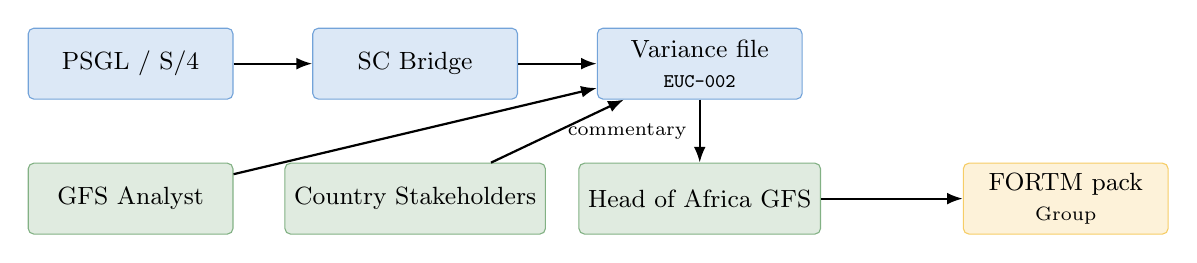
\begin{tikzpicture}[
node distance=8mm and 10mm,
box/.style={draw,rounded corners=2pt,minimum height=9mm,minimum width=26mm,
align=center,font=\small},
sys/.style={box,fill=tbblue!15,draw=tbblue!60},
ppl/.style={box,fill=tbgreen!15,draw=tbgreen!60},
outp/.style={box,fill=tbamber!15,draw=tbamber!60},
arr/.style={-{Latex[length=2mm]},thick}
]
\node[sys] (psgl)   {PSGL / S/4};
\node[sys,right=of psgl] (bridge) {SC Bridge};
\node[sys,right=of bridge] (xl)  {Variance file \\ \scriptsize \texttt{EUC-002}};
\node[ppl,below=of psgl] (gfs)   {GFS Analyst};
\node[ppl,below=of bridge] (cty) {Country Stakeholders};
\node[ppl,below=of xl]    (hd)   {Head of Africa GFS};
\node[outp,right=18mm of hd] (fortm) {FORTM pack \\ \scriptsize Group};

\draw[arr] (psgl)   -- (bridge);
\draw[arr] (bridge) -- (xl);
\draw[arr] (gfs)    -- (xl);
\draw[arr] (cty)    -- (xl) node[midway,right,font=\scriptsize]{commentary};
\draw[arr] (xl)     -- (hd);
\draw[arr] (hd)     -- (fortm);
\end{tikzpicture}
\caption{Context of the TB review process: three systems (blue), three
human roles (green), and one downstream output (amber). The
variance-analysis workbook is the primary EUC artefact.}\label{fig:context}
\end{figure}

\section{Expected benefits}

\begin{itemize}
\item FTE savings: 5 FTEs redeployed (business-case field
\texttt{executiveSummary.\allowbreak fteImpact.\allowbreak expectedSavings}).
\item Retirement of three EUCs (Group ACG alignment) on a
phased schedule: the three Excel-based EUCs
(\texttt{EUC-001}, \texttt{EUC-002}, \texttt{EUC-003}) are
replaced by the rule-firing log plus the review dashboard
audit trail (Chapter~\ref{ch:review-dashboard}). Shared
Drive evidence storage is retained only as a read-only
archive for a one-year deprecation window
(see Section~\ref{sec:euc-retirement-plan}); the dashboard
audit trail is the authoritative evidence source from
v1.0 cutover onwards.
\item Enablement of daily controls (from monthly batch).
\item Foundation for the SCB Finance LLM.
\end{itemize}

\section{EUC retirement plan}\label{sec:euc-retirement-plan}

The three EUCs are retired, not merely supplemented, on the
following schedule. ``Retirement'' means the EUC is no longer the
authoritative evidence for ACG sampling; the dashboard audit trail
(Chapter~\ref{ch:review-dashboard}, \cref{sec:dashboard-audit-trail}) is authoritative.

\begin{table}[htbp]
\centering
\caption{EUC retirement schedule.}
\label{tab:euc-retirement}
\footnotesize
\begin{tabularx}{\linewidth}{@{}l l l X@{}}
\toprule
\textbf{EUC} & \textbf{Artefact} & \textbf{Retirement cutover} & \textbf{Successor evidence} \\ \midrule
EUC-001 & PSGL master extract & Month of v1.0 go-live & Dashboard ``Master Data'' tab; SHA-256 of extract in audit trail \\
EUC-002 & Variance analysis workbook & Month of v1.0 go-live & Dashboard ``Variance Review'' tab; per-item decision record \\
EUC-003 & FORTM Pack & Month of v1.0 go-live + 1 cycle & Dashboard ``FORTM Export'' with signed PDF snapshot \\
\bottomrule
\end{tabularx}
\end{table}

\noindent
During the deprecation window (12 months from v1.0 go-live), the
Shared Drive evidence folder is mirrored automatically from the
dashboard export at month-end (read-only, with mismatch alerting).
After the deprecation window closes, the Shared Drive location is
decommissioned and removed from the ACG sampling procedure.
Section~\ref{sec:controls-eucs} in Chapter~6 is superseded by this
plan for all v1.0 and later cycles; the Chapter~6 text is retained
as a historical reference only.
\chapter{Canonical Data Schema}\label{ch:schema}

\section{Overview}

Every artefact under review is represented by a JSON record validated
against a Draft-07 JSON Schema. Six schemas are defined; collectively
they constitute the data contract consumed by the AI pipeline
(\cref{ch:ai}) and by the controls engine (\cref{ch:controls-engine}).

\begin{table}[htbp]
\caption{Schemas under \texttt{structured/schema/}.}\label{tab:schemas}
\centering
\small
\begin{tabularx}{\linewidth}{@{}lXr@{}}
\toprule
\textbf{Schema} & \textbf{Validates} & \textbf{Records} \\ \midrule
\path{control.schema.json}         & EUC and process controls            & 3 \\
\path{decision-point.schema.json}  & Gateway logic records                & 5 \\
\path{workflow.schema.json}        & State machine for a TB workflow      & 1 \\
\path{requirement.schema.json}     & Business-case requirement            & 1 \\
\path{kpi.schema.json}             & KPI definitions (collection file)    & 6 \\
\path{glossary.schema.json}        & Domain glossary                      & 1 (28 terms) \\
\path{data-product.schema.json}    & ODPS 4.1 data-product manifest       & 1 \\
\bottomrule
\end{tabularx}
\end{table}

\section{Control record}\label{sec:control-schema}

A \texttt{control} binds a governance reference (the EUC identifier) to
one or more workflow states. It declares type, frequency, owner, and
the evidence location examined at audit.

\begin{table}[htbp]
\caption{\texttt{control.schema.json} fields.}\label{tab:control-fields}
\centering
\small
\begin{tabularx}{\linewidth}{@{}lllX@{}}
\toprule
\textbf{Field} & \textbf{Type} & \textbf{Req} & \textbf{Notes} \\ \midrule
controlId        & string  & Y & \texttt{EUC-\textit{nnn}} \\
eucReference     & string  & N & \texttt{EX/nnn/nnnnnnn/nnnn/nnn} pattern \\
controlObjective & string  & Y & Plain-language objective \\
controlType      & enum    & Y & \textsc{preventive}, \textsc{detective}, \textsc{corrective} \\
frequency        & enum    & Y & \textsc{daily}..\textsc{annually} \\
timing           & string  & N & \texttt{M$\pm$n} phase \\
owner            & string  & Y & GFS role or named individual \\
evidenceLocation & string  & N & Where audit evidence lives \\
relatedStates    & array   & Y & Workflow \texttt{stateId}s ($\ge$1) \\
workflowRef      & string  & N & Workflow \texttt{workflowId} \\
source\_document & object  & N & Path, optional page and sha256 \\
\bottomrule
\end{tabularx}
\end{table}

\begin{figure}[htbp]
\begin{lstlisting}[language=jsonx,caption={\texttt{EUC-002} variance-file
control record (abbreviated).},label=lst:euc-002]
{
"controlId": "EUC-002",
"eucReference": "EX/200/1579702/0001/000",
"controlObjective": "TB Variance Analysis file integrity and calculation accuracy",
"controlType": "detective",
"frequency": "monthly",
"timing": "M-2 to M+5",
"owner": "GFS Analyst",
"evidenceLocation": "Shared Drive",
"relatedStates": ["UPDATE_TB_DETAILS", "CALCULATE_VARIANCE", "FILTER_VARIANCES"],
"description": "Ensures variance calculations in the Excel working file are accurate."
}
\end{lstlisting}
\end{figure}

\section{Decision-point record}\label{sec:decision-point-schema}

A decision point encodes an exclusive gateway: an input metric, an
operator, a threshold (where applicable), and an enumerated list of
outcomes. Each outcome pairs a human-readable condition with a
machine-actionable \texttt{action} verb. The \texttt{aiAugmentation}
block names the substitution target for the manual judgement.

\begin{figure}[htbp]
\begin{lstlisting}[language=jsonx,caption={\texttt{DP-001} material
variance gateway.},label=lst:dp-001]
{
"id": "DP-001",
"name": "Material Variance Check",
"stateRef": "CHECK_MATERIAL_VARIANCES",
"inputMetric": "variance_amount",
"operator": "exceeds_threshold",
"threshold": "materiality_limit",
"outcomes": [
{ "condition": "Variances Are Material",  "action": "seek_commentaries" },
{ "condition": "Variances Not Material",  "action": "proceed_to_unexplained_check" }
],
"aiAugmentation": {
"opportunity": "Auto-classify variance materiality using ML threshold tuning.",
"dataNeeded": ["variance_amount", "account_category", "historical_thresholds"]
}
}
\end{lstlisting}
\end{figure}

\section{Workflow record}\label{sec:workflow-schema}

The workflow record declares a state machine. Valid \texttt{type}
values are \textsc{start\_event}, \textsc{end\_event}, \textsc{task},
\textsc{gateway\_exclusive}, \textsc{gateway\_parallel}, and
\textsc{intermediate\_event}. Each state carries optional
\texttt{systems}, \texttt{inputs}, \texttt{outputs}, a
\texttt{participant}, and a list of \texttt{transitions}. A transition
in a gateway state additionally carries a \texttt{condition} string
that matches one of the outcome labels in the associated decision
point.

\begin{table}[htbp]
\caption{Workflow state-machine header fields.}\label{tab:workflow-fields}
\centering
\small
\begin{tabularx}{\linewidth}{@{}lllX@{}}
\toprule
\textbf{Field} & \textbf{Type} & \textbf{Req} & \textbf{Notes} \\ \midrule
workflowId    & string & Y & Canonical slug (\texttt{tb-review-glo}) \\
version       & string & Y & SemVer \\
title         & string & Y & Long name \\
processOwner  & string & N & Named owner \\
timeline      & array  & N & Phase / timing / description \\
states        & array  & Y & $\ge 2$ states, including one \textsc{start\_event} and one \textsc{end\_event} \\
dataObjects   & array  & N & Workflow-scoped artefacts \\
participants  & array  & N & Roles and groups \\
\bottomrule
\end{tabularx}
\end{table}

\section{Requirement record}\label{sec:requirement-schema}

The requirement record captures the business case. It is scoped by a
status enum (\textsc{draft}, \textsc{review}, \textsc{approved},
\textsc{rejected}, \textsc{superseded}), contains executive summary,
scope, stakeholders, process steps (each with an \texttt{aiPriority}
enum from \textsc{low}..\textsc{critical}), decision points, KPI
references, control references, risk assessment, and a phased
implementation plan. The single record populated here is
\texttt{TB-REQ-001} in state \textsc{approved}.

\section{KPI record}\label{sec:kpi-schema}

KPIs are stored as a collection file at
\corpus\texttt{structured/kpis/tb-kpis.json} containing one array
entry per KPI (\cref{tab:kpis}). Each entry is validated against
\path{kpi.schema.json}; the wrapper is checked by
\path{structured/validate.py}.

\begin{table}[htbp]
\caption{The six KPIs defined for the TB process.}\label{tab:kpis}
\centering
\small
\begin{tabularx}{\linewidth}{@{}llXl@{}}
\toprule
\textbf{KPI} & \textbf{Type} & \textbf{Description} & \textbf{Target} \\ \midrule
TB-KPI-001 & threshold  & Variance materiality threshold       & country-specific \\
TB-KPI-002 & duration   & TB review cycle time                 & reduce via daily controls \\
TB-KPI-003 & percentage & Commentary coverage                  & 100 \\
TB-KPI-004 & effort     & FTE effort                           & 15--20 FTEs \\
TB-KPI-005 & percentage & Unexplained variance rate            & 0 \\
TB-KPI-006 & percentage & EUC control compliance               & 100 \\
\bottomrule
\end{tabularx}
\end{table}

\section{Glossary record}

One glossary record contains 28 terms drawn verbatim from the
business case and the DOI. Category membership
(\textsc{balance\_sheet}, \textsc{income\_statement}, \textsc{general},
\textsc{regulatory}) is used by the GlossaryService pair-type alias
expansion at query time.

\section{Data-product record}

The data-product record is an ODPS 4.1-conformant manifest. It names
the routing policy (\texttt{vllm-only}), the data security class
(\textsc{confidential}), the owner, the per-country view for HK, the
system prompt, and the RAG source wiring. Consumers read this record
to know whether a given user request is permitted to contact external
LLM providers --- the answer for all TB artefacts is \emph{no}.

\section{Enumerations}

All enumerated values used in any schema or record are listed
authoritatively in \corpus\texttt{structured/enums.yaml}.
\Cref{tab:enums} summarises the most frequently referenced groups.

\begin{table}[htbp]
\caption{Frequently referenced enumerations.}\label{tab:enums}
\centering
\small
\begin{tabularx}{\linewidth}{@{}lX@{}}
\toprule
\textbf{Enum} & \textbf{Values} \\ \midrule
control\_type        & preventive, detective, corrective \\
workflow\_state\_type & start\_event, end\_event, task, gateway\_exclusive, gateway\_parallel, intermediate\_event \\
decision\_operator   & equals, not\_equals, exceeds\_threshold, within\_threshold, in\_set, boolean \\
ai\_priority         & low, medium, high, critical \\
risk\_severity       & L, M, H \\
kpi\_measure\_type    & threshold, duration, percentage, effort, count, ratio \\
data\_security\_class & public, internal, confidential, restricted \\
\bottomrule
\end{tabularx}
\end{table}

\section{Validation}

A local registry-based validator is provided at
\corpus\texttt{structured/validate.py}. It walks the record
directories, maps each to its schema via
\path{RECORD_DIRS}, and reports per-file results. The script is
offline: it instantiates a \texttt{referencing.Registry} loaded from
\corpus\texttt{structured/schema/} so no network resolution is
attempted.

\begin{lstlisting}[caption={Running the validator.},label=lst:validate]
$ python3 docs/tb/structured/validate.py
[ok]   controls/euc-001-tb-data-extraction.json
[ok]   controls/euc-002-variance-analysis-file.json
[ok]   controls/euc-003-internal-review.json
[ok]   decision-points/dp-001-material-variance.json
...
[ok]   corpus.json (17 items, all paths resolved)
13/13 records validated, corpus OK
\end{lstlisting}

\section{Unified Schema Registry}

As of 18 April 2026, all schemas in this specification are published in the
unified schema registry at \path{docs/schema/}. Migration status is
\emph{complete} (see \path{docs/schema/registry.json} field
\texttt{migration.status}). This consolidation addresses cross-document schema
divergence identified in the specification review.

\begin{description}
\item[Registry index.] \path{docs/schema/registry.json} --- Master index of
all schemas across domains.
\item[Common types.] \path{docs/schema/common/base-types.schema.json} ---
Shared definitions (\texttt{Metadata}, \texttt{Currency},
\texttt{DateRange}) referenced via JSON Schema \texttt{\$ref}.
\item[Consolidated enums.] \path{docs/schema/common/enums.yaml} --- Single
source of truth for enumeration values including \texttt{account\_category},
\texttt{variance\_flag}, \texttt{decision\_point}, and
\texttt{workflow\_status}.
\item[TB schemas.] \path{docs/schema/tb/} --- Domain-specific schemas:
\texttt{tb-extract.schema.json}, \texttt{pl-extract.schema.json},
\texttt{variance-record.schema.json}, \texttt{commentary-draft.schema.json},
and \texttt{decision-point.schema.json}. All marked \texttt{status: stable}.
\end{description}

\noindent
The legacy YAML schemas at \path{docs/tb/machine-readable/training-data/hkg-tb-schema.yaml}
and \path{docs/tb/machine-readable/training-data/hkg-pl-schema.yaml} have been
converted to JSON Schema Draft-07 in the unified registry; the registry
entries record the \texttt{legacy\_path} for audit traceability. The legacy
files are retained read-only during a one-release deprecation window and
will be removed in v1.1. Validation:

\begin{lstlisting}[language=bash]
python3 docs/schema/validate.py --registry-check
python3 docs/schema/validate.py --domain tb \
--schema tb-extract.schema.json --file tb-hkg-2026-03.json
\end{lstlisting}

\noindent
CI runs \texttt{--registry-check} on every pull request that touches
\path{docs/schema/} or any TB pipeline module.
\chapter{AI Augmentation Pipeline}\label{ch:ai}

\section{Architecture}

The AI pipeline is a five-stage request-response chain, hosted on the
internal vLLM cluster per the \texttt{vllm-only} routing policy in
\path{docs/tb/structured/data-products/trial-balance-review-v1.json}.
Every stage reads and writes records validated by \cref{ch:schema};
no blob passes between stages without a schema binding.

\begin{figure}[htbp]
\centering
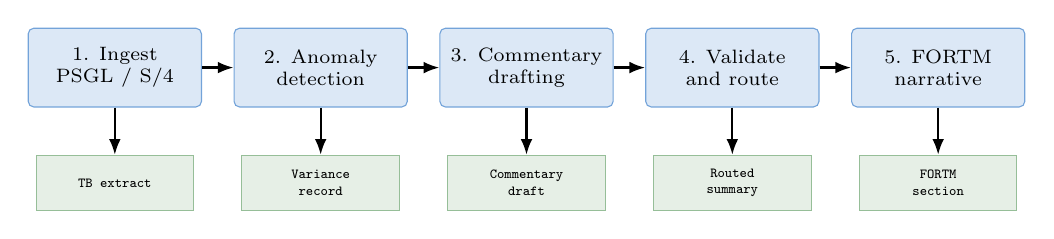
\begin{tikzpicture}[
node distance=6mm and 4mm,
stage/.style={draw,rounded corners=2pt,minimum height=10mm,
minimum width=22mm,align=center,font=\scriptsize,
fill=tbblue!15,draw=tbblue!60},
io/.style={draw,minimum height=7mm,minimum width=20mm,
align=center,font=\tiny\ttfamily,
fill=tbgreen!12,draw=tbgreen!50},
arr/.style={-{Latex[length=2mm]},thick}
]
\node[stage] (ingest)  {1. Ingest \\ \scriptsize PSGL / S/4};
\node[stage,right=of ingest]  (anomaly) {2. Anomaly \\ detection};
\node[stage,right=of anomaly] (commentary) {3. Commentary \\ drafting};
\node[stage,right=of commentary] (validate) {4. Validate \\ and route};
\node[stage,right=of validate]  (narrative) {5. FORTM \\ narrative};

\node[io,below=of ingest]     (rec1) {TB extract};
\node[io,below=of anomaly]    (rec2) {Variance \\ record};
\node[io,below=of commentary] (rec3) {Commentary \\ draft};
\node[io,below=of validate]   (rec4) {Routed \\ summary};
\node[io,below=of narrative]  (rec5) {FORTM \\ section};

\foreach \a/\b in {ingest/anomaly,anomaly/commentary,
commentary/validate,validate/narrative}
\draw[arr] (\a) -- (\b);
\foreach \s/\r in {ingest/rec1,anomaly/rec2,commentary/rec3,
validate/rec4,narrative/rec5}
\draw[arr] (\s) -- (\r);
\end{tikzpicture}
\caption{Five-stage AI pipeline; each stage emits a schema-bound
artefact.}\label{fig:ai-pipeline}
\end{figure}

\section{Stage 1: Ingestion}

\begin{description}
\item[Input.] PSGL master account data and the SC~Bridge TB
extract, one per LE, keyed on the \texttt{UPDATE\_TB\_DETAILS}
workflow state.
\item[Transform.] Column normalisation against
\path{docs/tb/machine-readable/training-data/hkg-tb-schema.yaml}
(13 sheets). Bank CSV samples live in
\path{docs/tb/extracted-text/hkg-tb-sample.csv} and
\path{docs/tb/extracted-text/hkg-pl-sample.csv}.
\item[Acceptance.] \texttt{EUC-001} evidence rules apply: the
extraction must preserve debit/credit totals and every row
must carry a valid account number from the refreshed master.
\end{description}

\section{Stage 2: Anomaly detection}

The anomaly detector performs four orthogonal checks per account
(\cref{tab:anomalies}). Thresholds are account-category-sensitive and
are re-fit monthly from the prior twelve months; the fitted thresholds
are persisted to the variance file EUC as audit evidence.

\begin{table}[htbp]
\caption{Anomaly checks run per account.}\label{tab:anomalies}
\centering
\small
\begin{tabularx}{\linewidth}{@{}llX@{}}
\toprule
\textbf{Check} & \textbf{Metric} & \textbf{Rule} \\ \midrule
Period spike   & $|\Delta|$       & $> 3\sigma$ over prior 12 months$^{\dagger}$ \\
Sign flip       & sign($v_t$)       & $\neq$ sign($v_{t-1}$) and $|v_t| > $ threshold \\
New account     & existence         & account absent from prior-period master \\
Stale balance   & $|\Delta|$        & $= 0$ for $\ge 3$ consecutive periods with prior activity \\
\bottomrule
\end{tabularx}
\end{table}

\noindent$^{\dagger}$\textbf{Assumption caveat:} The $3\sigma$ threshold assumes
normally-distributed variance values. This assumption has not been statistically
validated against the TB population; financial data often exhibits fat tails
(leptokurtosis). The pilot will include a Shapiro-Wilk normality test per account
category. Non-normal distributions may require robust alternatives (e.g., MAD-based
z-scores or quantile thresholds). Thresholds marked ``TBD pending pilot.''

Only accounts flagged by at least one check enter Stage 3. Accounts
below materiality (\texttt{DP-001}) are still logged for audit but
short-circuit to Stage 4.

\section{Stage 3: Commentary drafting}

\paragraph{Model.} A vLLM-hosted instruction-tuned model accessed
via the internal gateway. The system prompt is the
\texttt{x-prompting-policy.systemPrompt} field of the data product
record; \texttt{maxTokens = 4096}, \texttt{temperature = 0.3},
\texttt{responseFormat = "text"}.

\paragraph{Prompt structure.} Each commentary request carries:
\begin{itemize}
\item The flagged variance record (account, prior, current, delta).
\item The three most similar historical commentaries retrieved from
the \texttt{TB\_REVIEW\_VECTORS} table (55 chunks, 220-word
chunking with 40-word overlap; see
\corpus\texttt{machine-readable/rag/rag\_embedding\_records.jsonl}).
\item The account's finance caption and segment.
\item Any related journal identifiers found in the GL for the period.
\end{itemize}

\paragraph{Output contract.} The draft is returned as a
\texttt{commentary\_draft} blob that is paired with the variance
record before leaving the stage. Human review by the GFS Analyst is
mandatory (per DOI \texttt{REVIEW\_INCORPORATE}); the draft is a
\emph{suggestion}, never a final artefact.

\section{Stage 4: Validation and routing}

The gateway logic defined in \cref{ch:workflow} is evaluated here.
\Cref{tab:routing} maps each decision point to the record fields the
engine reads.

\begin{table}[htbp]
\caption{Decision-point routing.}\label{tab:routing}
\centering
\small
\begin{tabularx}{\linewidth}{@{}llX@{}}
\toprule
\textbf{DP} & \textbf{Gateway state} & \textbf{Read fields} \\ \midrule
DP-001 & CHECK\_MATERIAL\_VARIANCES & variance\_amount, account\_category, materiality\_limit \\
DP-002 & IS\_JOURNAL\_POSTED         & journal\_status, posting\_date \\
DP-003 & CHECK\_FURTHER\_INVESTIGATION & investigation\_status, entry\_age\_days \\
DP-004 & CHECK\_CONFIRMATION         & confirmation\_received, days\_to\_deadline (M+4) \\
DP-005 & CHECK\_UNEXPLAINED          & unexplained\_variance\_count \\
\bottomrule
\end{tabularx}
\end{table}

\section{Stage 5: FORTM narrative generation}

The final stage composes the FORTM pack section. It consumes the
routed summary plus the KPI telemetry (\cref{tab:kpis}) and emits a
structured narrative containing: executive summary, material variance
table, unexplained items, risk register update, and the list of
outstanding journal postings. The narrative goes to
\stateid{REVIEW\_INCORPORATE} for \texttt{EUC-003} sign-off before
\stateid{SEND\_FORTM}.

\section{Controls posture of the pipeline}

Every stage is in-scope of the UK ACG automated-controls regime. The
per-stage control posture is summarised in \cref{tab:ai-controls}.

\begin{table}[htbp]
\caption{Per-stage controls posture.}\label{tab:ai-controls}
\centering
\small
\begin{tabularx}{\linewidth}{@{}llX@{}}
\toprule
\textbf{Stage} & \textbf{Control type} & \textbf{Mechanism} \\ \midrule
Ingest        & preventive & Totals reconciliation vs PSGL source \\
Anomaly       & detective  & Threshold log + human sampling \\
Commentary    & detective  & Mandatory human review (DOI) \\
Validation    & preventive & Schema + gateway enforcement \\
FORTM         & detective  & EUC-003 senior sign-off \\
\bottomrule
\end{tabularx}
\end{table}

\section{Evaluation harness}

\begin{description}
\item[Golden set.] The HK Nov~2025 workbooks
(\corpus\texttt{source/HKG\_TB review Nov'25.xlsm} and
\corpus\texttt{source/HKG\_PL review Nov'25.xlsm}) serve as
regression data. All 234 LEs enter at phase~4 of the
implementation plan.
\item[Commentary metric.] Draft quality is scored against analyst
accepts in the DOI review phase; target accept-without-edit
$\ge$ 70\%, accept-with-edit $\ge$ 95\%.
\item[Anomaly metric.] Per-check precision/recall against analyst
flags in a held-out period.
\item[Cycle time.] Measured as \texttt{TB-KPI-002}; target is the
enablement of a daily cadence, which collapses the cycle from
\texttt{M+1..M+7} to a rolling one-day delay.
\end{description}
\chapter{Controls and Commentary Engine}\label{ch:controls-engine}

\section{Role of the engine}

The controls engine is the declarative layer that turns the five
decision-point records of \cref{sec:decision-point-schema} into
executable rules. It sits between Stage 2 (anomaly detection) and
Stage 5 (FORTM narrative) of the AI pipeline. Its inputs are the
variance records, the GL journal extract, and the stakeholder
commentary responses; its outputs are routing actions and a
commentary register.

\section{Decision tree}

\Cref{fig:decision-tree} collapses the five gateways into a single
cascade. The tree is identical to the workflow in \cref{ch:workflow}
but omits task nodes; each leaf is a terminal action in the gateway
vocabulary.

\begin{figure}[htbp]
\centering
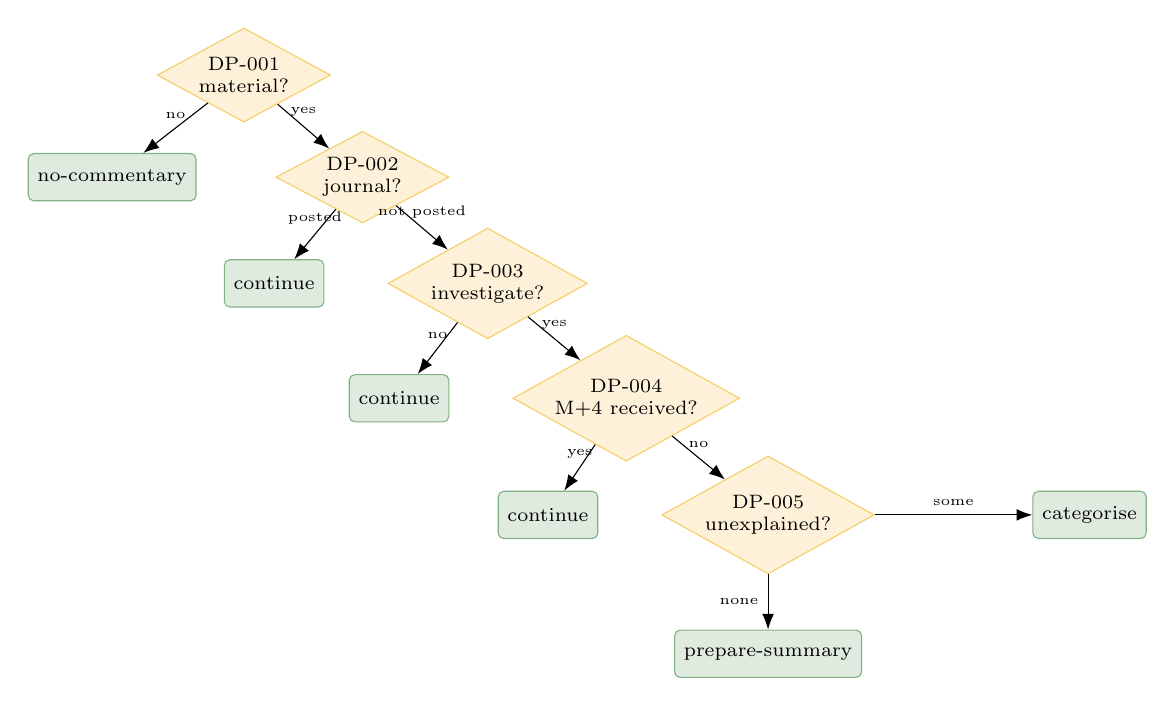
\begin{tikzpicture}[
node distance=7mm and 8mm,
gw/.style={diamond,draw,aspect=1.8,inner sep=1pt,align=center,
font=\scriptsize,fill=tbamber!15,draw=tbamber!60,
minimum height=9mm,minimum width=22mm},
act/.style={draw,rounded corners=2pt,align=center,font=\scriptsize,
fill=tbgreen!15,draw=tbgreen!60,minimum height=6mm},
arr/.style={-{Latex[length=2mm]},thin}
]
\node[gw] (dp1) {DP-001 \\ material?};
\node[gw,below right=7mm and 4mm of dp1] (dp2) {DP-002 \\ journal?};
\node[act,left=10mm of dp2] (noncrit) {no-commentary};
\node[gw,below right=7mm and 4mm of dp2] (dp3) {DP-003 \\ investigate?};
\node[act,left=8mm of dp3] (posted) {continue};
\node[gw,below right=7mm and 4mm of dp3] (dp4) {DP-004 \\ M+4 received?};
\node[act,left=8mm of dp4] (norinv) {continue};
\node[gw,below right=7mm and 4mm of dp4] (dp5) {DP-005 \\ unexplained?};
\node[act,left=8mm of dp5] (ontime) {continue};
\node[act,below=of dp5] (summary) {prepare-summary};
\node[act,right=20mm of dp5] (cat) {categorise};

\draw[arr] (dp1) -- node[above,font=\tiny]{yes} (dp2);
\draw[arr] (dp1) -- node[above,font=\tiny]{no}  (noncrit);
\draw[arr] (dp2) -- node[above,font=\tiny]{not posted} (dp3);
\draw[arr] (dp2) -- node[above,font=\tiny]{posted}     (posted);
\draw[arr] (dp3) -- node[above,font=\tiny]{yes} (dp4);
\draw[arr] (dp3) -- node[above,font=\tiny]{no}  (norinv);
\draw[arr] (dp4) -- node[above,font=\tiny]{no}  (dp5);
\draw[arr] (dp4) -- node[above,font=\tiny]{yes} (ontime);
\draw[arr] (dp5) -- node[left,font=\tiny]{none}  (summary);
\draw[arr] (dp5) -- node[above,font=\tiny]{some} (cat);
\end{tikzpicture}
\caption{Decision cascade encoded by the five decision-point
records.}\label{fig:decision-tree}
\end{figure}

\section{Rule format}

Each rule is a record with five fields:

\begin{lstlisting}[language=jsonx,caption={Generalised rule form.}]
{
"id":          "<DP-nnn>",
"state":       "<workflow stateId>",
"input":       "<record field path>",
"operator":    "<exceeds_threshold|boolean|in_set|...>",
"threshold":   "<value or parameter name>",
"branches":    [ {"condition":"...","action":"..."} ... ]
}
\end{lstlisting}

Rule evaluation is deterministic. When a record enters a gateway
state, the engine reads the named input field, applies the operator,
and dispatches the matching branch's action. Actions reference
downstream tasks in the workflow (\cref{ch:workflow}).

\section{Materiality thresholds}

\texttt{DP-001} reads \texttt{materiality\_limit} from the country
parameters sheet. During the AI rollout, the fitted ML threshold
(Stage 2) is compared side-by-side with the manual limit for six
months; divergences $> 10\%$ surface to the Head of Africa GFS for
review. Only after six clean cycles does the fitted threshold
replace the manual one in the parameter sheet.

\section{Journal posting}

\texttt{DP-002} has three branches. The engine first reads
\texttt{journal\_status} from the GL extract. If the status is
\textsc{posted}, the routing short-circuits to
\stateid{CHECK\_UNEXPLAINED}. If \textsc{posting\_required}, the
engine emits a posting request via
\stateid{SEND\_JOURNAL\_REQUEST} and returns to
\stateid{CHECK\_FURTHER\_INVESTIGATION}. If \textsc{not\_posted}
(stuck), the path proceeds directly to
\stateid{CHECK\_FURTHER\_INVESTIGATION}, skipping the request.

\section{Investigation and deadlines}

\texttt{DP-003} is a boolean gateway controlled by the
\texttt{investigation\_status} field. \texttt{DP-004} enforces the
\texttt{M+4} deadline by reading \texttt{days\_to\_deadline} from the
variance record. Crossing the deadline triggers the
\stateid{TRACK\_ENTRIES} branch and the risk-assessment update in
\stateid{UPDATE\_RISK}.

\section{Unexplained-variance handling}

\texttt{DP-005} is the final gate before summary. If
\texttt{unexplained\_variance\_count $= 0$}, the engine transitions to
\stateid{PREPARE\_SUMMARY}. Otherwise, the unexplained items are
passed to \stateid{CATEGORIZE\_UNEXPLAINED}, where each item is
tagged against the BSS risk vocabulary (\textsc{substantiated at risk},
\textsc{unsubstantiated unowned}, \textsc{unsubstantiated owned}) and
a commentary draft is requested.

\section{Commentary register}

All drafts produced by Stage 3 of the AI pipeline, together with the
analyst accept/edit decision, are persisted to the commentary
register. The register is the primary evidence artefact for
\texttt{EUC-002}: the register row count must equal the flagged
variance row count at the end of \stateid{UPDATE\_VARIANCE\_COMMENTARIES}.

\begin{table}[htbp]
\caption{Commentary register schema (derived from the variance
record).}\label{tab:commentary-register}
\centering
\small
\begin{tabularx}{\linewidth}{@{}llX@{}}
\toprule
\textbf{Field} & \textbf{Type} & \textbf{Notes} \\ \midrule
account\_id      & string  & GL account number \\
period           & string  & ISO yyyy-mm \\
variance\_amount & number  & Prior $\to$ current delta \\
draft            & string  & LLM-generated narrative \\
final            & string  & Post-review narrative \\
accept\_mode     & enum    & \textsc{as-is}, \textsc{edited}, \textsc{rejected} \\
reviewer         & string  & GFS Analyst name or role \\
review\_ts       & datetime & ISO-8601 \\
\bottomrule
\end{tabularx}
\end{table}

\section{Per-country parameter views}\label{sec:per-country-views}

The data product record carries a \texttt{x-country-views.HK} block
that injects an HKMA-aware vocabulary and sets
\texttt{defaultFilters.entity = "HKG"}. Adding a new country is a
matter of adding another view; no schema change is needed. Until
additional views exist, Hong Kong is the only LE with a fitted
threshold history.

\subsection{Parameter loading and validation for 234 entities}
\label{sec:params-234}

Full Group rollout to all 234 Legal Entities (LEs) is gated on the
availability of a per-entity parameter file, not on model capacity.
This section specifies how those parameters are loaded, validated,
and versioned so that entities can be on-boarded without schema or
code changes.

\begin{description}
\item[Parameter file layout.] Per-entity parameters live at
\path{docs/tb/machine-readable/entity-params/<le-code>.yaml}
(one file per LE; \texttt{le-code} matches the three-letter
ISO-ish LE code used by PSGL, e.g.\ \texttt{HKG},
\texttt{SGP}). Each file is a dictionary with keys
\texttt{materiality\_threshold}, \texttt{variance\_bands},
\texttt{account\_category\_overrides},
\texttt{fx\_reporting\_currency},
\texttt{regulator\_vocabulary},
\texttt{commentary\_style\_exemplars}, and
\texttt{last\_calibration\_date}.
\item[Schema.] All entity parameter files validate against
\path{docs/schema/tb/entity-params.schema.json} (new,
registered in \path{docs/schema/registry.json} under the
\texttt{tb} domain). The CI \texttt{--registry-check}
command fails if any file deviates.
\item[Loading.] The TB pipeline loads parameters at batch start
via \texttt{EntityParamsRegistry.load\_all()}
(\path{src/tb/entity_params.py}) which reads every file in
the directory, validates it against the schema, and caches
the result. Missing LE codes are logged as
\texttt{warn}; a missing code does not block the pipeline
for \emph{other} entities, but processing for the missing
LE is skipped with an audit record.
\item[Onboarding a new LE.] The runbook is
\path{docs/tb/runbooks/onboard-le.md}: (1) copy
\texttt{HKG.yaml} as a template, (2) fit a threshold
history against 12 months of TB data, (3) open a pull
request with the new file, (4) CI validates the file and
runs a dry-run cycle on the new LE, (5) reviewer sign-off
(senior analyst + controller).
\item[Roll-forward safety.] Parameter files are versioned in
git; the data product record records the git SHA of the
entity-params directory at run start
(\texttt{runMetadata.entityParamsSha}). Retrospective
ACG queries reconstruct parameters at the historical run
time.
\end{description}

\noindent
Rollout readiness (see Chapter~\ref{ch:overview}, Section on
Timeline): HKG is fully onboarded; a wave of 8--10 LEs is added in
phase~4 (quarter after v1.0 go-live), with the remaining 220+
on-boarded over 12--18 months. The dashboard
(\cref{ch:review-dashboard}) surfaces per-LE coverage so that
operations can prioritise LEs by review volume and regulator risk.

\section{Observability}

Every rule firing is logged with input, branch taken, timestamp, and
the version of the ruleset. Logs are aggregated into the
\texttt{TB\_REVIEW\_VECTORS} table's metadata index so that prior
decisions are retrievable by account and period.
\chapter{Workflow and Approval Engine}\label{ch:workflow}

\section{Source}

The workflow engine formalises the 28-state BPMN diagram captured in
\corpus\texttt{structured/workflows/tb-review-glo.json}. The diagram
is derived from two source artefacts:

\begin{itemize}
\item \corpus\texttt{source/Operation of Month End Close Controls\ \ - Trial Balance Review - GLO (1).pdf}
--- the control narrative that defines the seven DOI activities,
\item \corpus\texttt{source/Business case - Trial Balance (2).doc}
--- the business case that expands the activities into the
eight process steps of \texttt{TB-REQ-001}.
\end{itemize}

\section{State inventory}

\Cref{tab:states} enumerates the 28 states. Tasks are numbered
sequentially; gateways and events are marked in the \textbf{Type}
column.

\begin{table}[htbp]
\caption{States in \texttt{tb-review-glo} (28 in total).}\label{tab:states}
\centering
\footnotesize
\begin{tabularx}{\linewidth}{@{}llllX@{}}
\toprule
\textbf{\#} & \textbf{State ID} & \textbf{Type} & \textbf{Timing} & \textbf{Name} \\ \midrule
1  & START                         & start        & ---        & Prepare Schedule Work Day \\
2  & ROLL\_FORWARD                 & task         & M-3        & Roll Forward Prior Month File \\
3  & DOWNLOAD\_PSGL                & task         & M-3        & Download PSGL Master Account File \\
4  & UPDATE\_ACCOUNTS\_MASTER      & task         & M-3        & Update Accounts Master Sheet \\
5  & UPDATE\_PARAMETERS            & task         & M-3        & Update Parameters and Comparatives \\
6  & EXTRACT\_TB                   & task         & M-3..M+5   & Extract Trial Balance \\
7  & UPDATE\_TB\_DETAILS           & task         & M-2..M+5   & Update TB Details (EUC-002) \\
8  & CALCULATE\_VARIANCE           & task         & M-2..M+5   & Calculate Variance \\
9  & FILTER\_VARIANCES             & task         & M-2..M+5   & Filter Variances \\
10 & CHECK\_MATERIAL\_VARIANCES    & gw-excl      & M-2..M+5   & Material variance? (DP-001) \\
11 & SEEK\_COMMENTARIES            & task         & M-2..M+5   & Seek Commentaries \\
12 & RECEIVE\_COMMENTARIES         & intermediate & M-2..M+5   & Receive Commentaries \\
13 & UPDATE\_COMMENTARIES          & task         & M-2..M+5   & Update Commentaries \\
14 & UPDATE\_VARIANCE\_COMMENTARIES & task        & M-2..M+5   & Finalise Commentaries \\
15 & IS\_JOURNAL\_POSTED           & gw-excl      & M-2..M+5   & Journal posted? (DP-002) \\
16 & SEND\_JOURNAL\_REQUEST        & task         & M-2..M+5   & Send Posting Request \\
17 & CHECK\_FURTHER\_INVESTIGATION & gw-excl      & M-2..M+5   & Investigate? (DP-003) \\
18 & CHECK\_ENTRIES\_STATUS        & task         & M-2..M+5   & Check with Team \\
19 & CHECK\_CONFIRMATION           & gw-excl      & M-2..M+5   & M+4 received? (DP-004) \\
20 & TRACK\_ENTRIES                & task         & M-2..M+5   & Track and Risk Analyse \\
21 & UPDATE\_RISK                  & task         & M-2..M+5   & Update Risk Assessment \\
22 & CHECK\_UNEXPLAINED            & gw-excl      & M-2..M+5   & Unexplained? (DP-005) \\
23 & CATEGORIZE\_UNEXPLAINED       & task         & M-2..M+5   & Categorise Unexplained \\
24 & PREPARE\_SUMMARY              & task         & M-2..M+5   & Prepare Summary \\
25 & SEND\_INTERNAL\_REVIEW        & task         & M+5        & Send for Internal Review \\
26 & REVIEW\_INCORPORATE           & task         & M+5        & Review (EUC-003) \\
27 & SEND\_FORTM                   & task         & M+5        & Send FORTM Summary \\
28 & END                           & end          & ---        & TB Review Completed \\
\bottomrule
\end{tabularx}
\end{table}

\section{Preparation phase (M-3)}

\Cref{fig:prep-phase} shows states 1--6. Execution is strictly
sequential; every state has exactly one outgoing transition.

\begin{figure}[htbp]
\centering
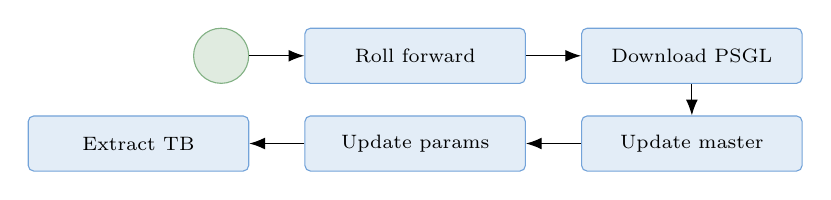
\begin{tikzpicture}[
node distance=4mm and 7mm,
task/.style={draw,rounded corners=2pt,align=center,font=\scriptsize,
fill=tbblue!12,draw=tbblue!60,minimum height=7mm,
minimum width=28mm},
ev/.style={circle,draw,align=center,font=\scriptsize,
fill=tbgreen!15,draw=tbgreen!60,minimum size=7mm},
arr/.style={-{Latex[length=2mm]},thin}
]
\node[ev]   (s) {};
\node[task,right=of s]         (rf) {Roll forward};
\node[task,right=of rf]        (dp) {Download PSGL};
\node[task,below=of dp]        (am) {Update master};
\node[task,left=of am]         (pa) {Update params};
\node[task,left=of pa]         (ex) {Extract TB};
\foreach \a/\b in {s/rf,rf/dp,dp/am,am/pa,pa/ex}
\draw[arr] (\a) -- (\b);
\end{tikzpicture}
\caption{Preparation phase (states 1--6). EUC-001 governs the PSGL
download and TB extraction steps.}\label{fig:prep-phase}
\end{figure}

\section{Analysis phase (M-2 to M+5)}

The analysis phase is the control-rich core of the process. It holds
all five gateways, all commentary handling, and the journal-posting
cycle. \Cref{fig:analysis-phase} shows states 7--24.

\begin{figure}[htbp]
\centering
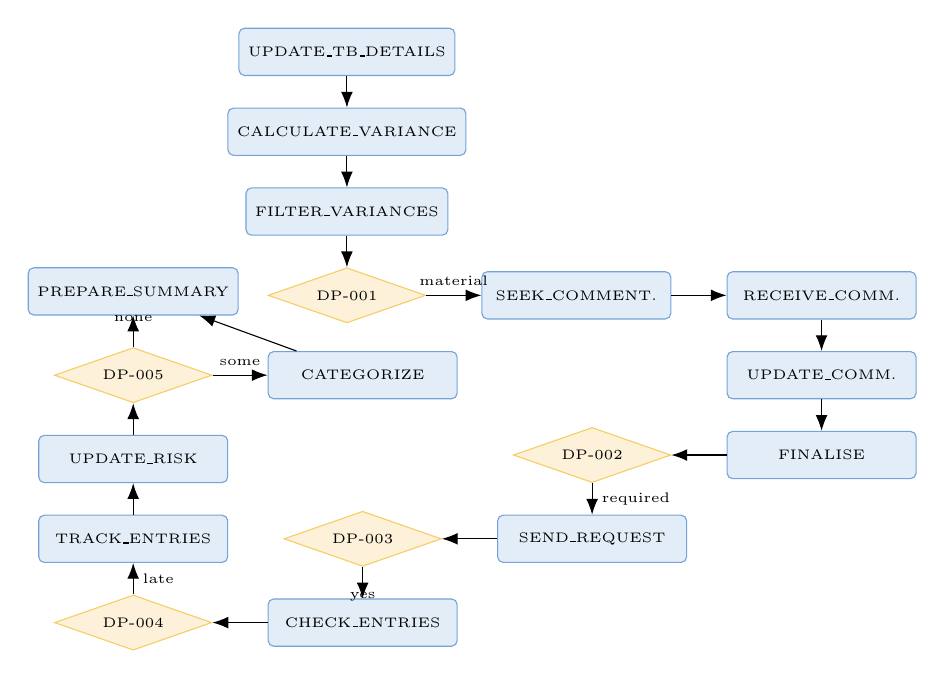
\begin{tikzpicture}[
node distance=4mm and 7mm,
task/.style={draw,rounded corners=2pt,align=center,font=\tiny,
fill=tbblue!12,draw=tbblue!60,minimum height=6mm,
minimum width=24mm},
gw/.style={diamond,draw,aspect=1.8,inner sep=1pt,align=center,
font=\tiny,fill=tbamber!15,draw=tbamber!60,
minimum height=7mm,minimum width=20mm},
arr/.style={-{Latex[length=2mm]},thin}
]
\node[task] (u)  {UPDATE\_TB\_DETAILS};
\node[task,below=of u] (c) {CALCULATE\_VARIANCE};
\node[task,below=of c] (f) {FILTER\_VARIANCES};
\node[gw,below=of f]   (m) {DP-001};
\node[task,right=of m] (sc) {SEEK\_COMMENT.};
\node[task,right=of sc] (rc) {RECEIVE\_COMM.};
\node[task,below=of rc] (uc) {UPDATE\_COMM.};
\node[task,below=of uc] (fc) {FINALISE};
\node[gw,left=of fc]   (j) {DP-002};
\node[task,below=of j] (sr) {SEND\_REQUEST};
\node[gw,left=of sr]   (inv) {DP-003};
\node[task,below=of inv] (ce) {CHECK\_ENTRIES};
\node[gw,left=of ce]   (cf) {DP-004};
\node[task,above=of cf] (tr) {TRACK\_ENTRIES};
\node[task,above=of tr] (ur) {UPDATE\_RISK};
\node[gw,above=of ur]   (un) {DP-005};
\node[task,right=of un] (cat) {CATEGORIZE};
\node[task,above=of un] (ps) {PREPARE\_SUMMARY};

\foreach \a/\b in {u/c,c/f,f/m}             \draw[arr] (\a) -- (\b);
\draw[arr] (m)  -- node[above,font=\tiny]{material} (sc);
\draw[arr] (sc) -- (rc);
\draw[arr] (rc) -- (uc);
\draw[arr] (uc) -- (fc);
\draw[arr] (fc) -- (j);
\draw[arr] (j)  -- node[right,font=\tiny]{required} (sr);
\draw[arr] (sr) -- (inv);
\draw[arr] (inv) -- node[below,font=\tiny]{yes} (ce);
\draw[arr] (ce)  -- (cf);
\draw[arr] (cf)  -- node[right,font=\tiny]{late} (tr);
\draw[arr] (tr)  -- (ur);
\draw[arr] (ur)  -- (un);
\draw[arr] (un)  -- node[above,font=\tiny]{none} (ps);
\draw[arr] (un)  -- node[above,font=\tiny]{some} (cat);
\draw[arr] (cat) -- (ps);
\end{tikzpicture}
\caption{Analysis phase. Gateways DP-001..DP-005 are diamond nodes;
commentary loop sits to the right of DP-001; journal-posting loop sits
below DP-002. Not all transitions are drawn; see the full JSON for
completeness.}\label{fig:analysis-phase}
\end{figure}

\section{Review phase (M+5)}

\begin{figure}[htbp]
\centering
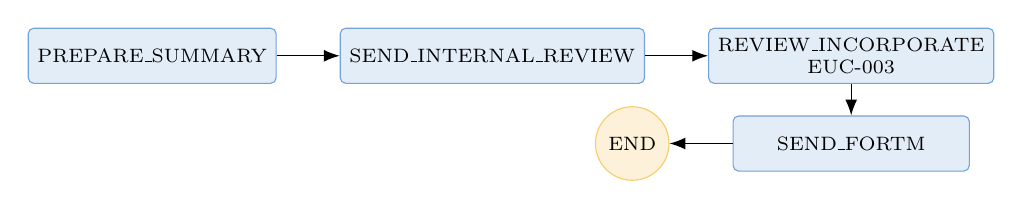
\begin{tikzpicture}[
node distance=4mm and 8mm,
task/.style={draw,rounded corners=2pt,align=center,font=\scriptsize,
fill=tbblue!12,draw=tbblue!60,minimum height=7mm,
minimum width=30mm},
ev/.style={circle,draw,align=center,font=\scriptsize,
fill=tbamber!15,draw=tbamber!60,minimum size=7mm},
arr/.style={-{Latex[length=2mm]},thin}
]
\node[task] (ps) {PREPARE\_SUMMARY};
\node[task,right=of ps] (si) {SEND\_INTERNAL\_REVIEW};
\node[task,right=of si] (ri) {REVIEW\_INCORPORATE \\ \scriptsize EUC-003};
\node[task,below=of ri] (sf) {SEND\_FORTM};
\node[ev,  left=of sf]  (e)  {END};
\foreach \a/\b in {ps/si,si/ri,ri/sf,sf/e}
\draw[arr] (\a) -- (\b);
\end{tikzpicture}
\caption{Review phase: senior sign-off (EUC-003) gates the FORTM
submission.}\label{fig:review-phase}
\end{figure}

\section{Approval matrix}

\begin{table}[htbp]
\caption{Approval and review responsibilities.}\label{tab:approval}
\centering
\small
\begin{tabularx}{\linewidth}{@{}llXl@{}}
\toprule
\textbf{State} & \textbf{Participant} & \textbf{Decision} & \textbf{Control} \\ \midrule
UPDATE\_TB\_DETAILS     & GFS Analyst        & File integrity            & EUC-002 \\
UPDATE\_COMMENTARIES    & GFS Analyst        & Draft accept/edit/reject  & ---      \\
REVIEW\_INCORPORATE     & Head of Africa GFS & Senior sign-off           & EUC-003 \\
SEND\_FORTM             & Head of Africa GFS & Release to Group          & ---      \\
\bottomrule
\end{tabularx}
\end{table}

\section{Data objects}

The five data objects declared on the workflow are listed in
\cref{tab:dataobjects}.

\begin{table}[htbp]
\caption{Workflow data objects.}\label{tab:dataobjects}
\centering
\small
\begin{tabularx}{\linewidth}{@{}llXl@{}}
\toprule
\textbf{ID} & \textbf{Name} & \textbf{Description} & \textbf{EUC} \\ \midrule
DO-001 & Variance Analysis File   & Primary working file              & EUC-002 \\
DO-002 & Shared Drive             & Evidence store                    & ---     \\
DO-003 & PSGL Master Account File & Master data extract               & EUC-001 \\
DO-004 & SC Bridge                & Extract interface                 & ---     \\
DO-005 & FORTM Pack               & Group-level reporting package     & EUC-003 \\
\bottomrule
\end{tabularx}
\end{table}

\section{Exception paths}

The workflow diagram encodes the happy path and the four
gateway-driven loops. Two operational exceptions are not drawn but
are handled by the engine:

\begin{enumerate}
\item \textbf{SC Bridge failure.} If \stateid{EXTRACT\_TB} cannot
read from the bridge, the state is parked and a human
notification is emitted. Re-entry resumes from
\stateid{EXTRACT\_TB}; earlier states are not replayed.
\item \textbf{Late FORTM change.} If Group requests a revision after
\stateid{END}, a new run is created with a suffix
\texttt{-revN}; evidence for the original run is retained.
\end{enumerate}
\chapter{Controls, Testing, and Acceptance}\label{ch:controls}

\section{Control enforcement map}

\Cref{fig:controls-map} binds each EUC control to the workflow states
it governs. The binding is authoritative: the
\texttt{relatedStates} array of each control record is the source of
truth.

\begin{figure}[htbp]
\centering
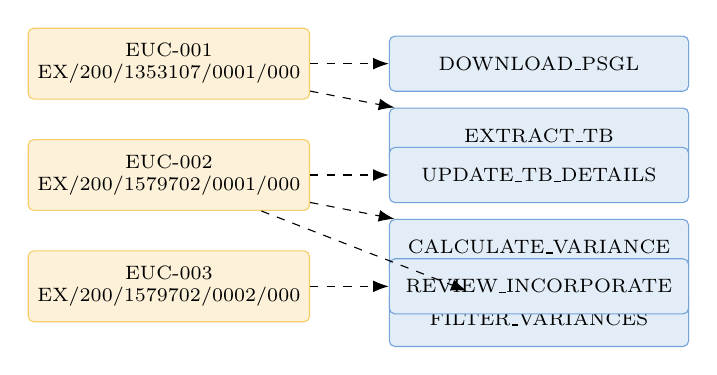
\begin{tikzpicture}[
node distance=5mm and 10mm,
ctrl/.style={draw,rounded corners=2pt,align=center,font=\scriptsize,
fill=tbamber!15,draw=tbamber!60,
minimum height=9mm,minimum width=32mm},
state/.style={draw,rounded corners=2pt,align=center,font=\scriptsize,
fill=tbblue!12,draw=tbblue!60,
minimum height=7mm,minimum width=38mm},
arr/.style={-{Latex[length=2mm]},thin,dashed}
]
\node[ctrl] (c1) {EUC-001 \\ \scriptsize EX/200/1353107/0001/000};
\node[ctrl,below=of c1] (c2) {EUC-002 \\ \scriptsize EX/200/1579702/0001/000};
\node[ctrl,below=of c2] (c3) {EUC-003 \\ \scriptsize EX/200/1579702/0002/000};

\node[state,right=of c1] (s1) {DOWNLOAD\_PSGL};
\node[state,below=2mm of s1] (s2) {EXTRACT\_TB};
\node[state,right=of c2] (s3) {UPDATE\_TB\_DETAILS};
\node[state,below=2mm of s3] (s4) {CALCULATE\_VARIANCE};
\node[state,below=2mm of s4] (s5) {FILTER\_VARIANCES};
\node[state,right=of c3] (s6) {REVIEW\_INCORPORATE};

\draw[arr] (c1) -- (s1);   \draw[arr] (c1) -- (s2);
\draw[arr] (c2) -- (s3);   \draw[arr] (c2) -- (s4);   \draw[arr] (c2) -- (s5);
\draw[arr] (c3) -- (s6);
\end{tikzpicture}
\caption{Control-to-state binding. Dashed lines denote the
\texttt{relatedStates} relation.}\label{fig:controls-map}
\end{figure}

\section{Risk register}

\Cref{tab:risks} lists the four control risks enumerated in
\path{docs/tb/machine-readable/process/tb-review-controls.yaml} and
the two business-case risks in
\path{docs/tb/structured/requirements/tb-business-requirements.json}.

\begin{table}[htbp]
\caption{Risks and mitigations.}\label{tab:risks}
\centering
\footnotesize
\begin{tabularx}{\linewidth}{@{}llXlX@{}}
\toprule
\textbf{ID} & \textbf{Severity} & \textbf{Description} & \textbf{Today} & \textbf{AI mitigation} \\ \midrule
CR-001       & high     & Manual extraction, EUC risk       & EUCs 001/002 & Fully automated ingest \\
CR-002       & medium   & Late commentary responses         & M+4 chasing  & Auto-drafts remove dependency \\
CR-003       & high     & Incomplete analysis under time pressure & 20--25 FTEs  & Parallel anomaly detection \\
CR-004       & medium   & Not scalable to daily ops         & none         & Foundation for daily cadence \\
TB-RISK-001  & H        & PSGL-only coverage today          & PSGL adapters only & Build S/4 adapter \\
TB-RISK-002  & H        & SAP integration dependency        & PPE review   & Compatibility assessment \\
\bottomrule
\end{tabularx}
\end{table}

\section{Test strategy}

Testing is layered; each layer has a named artefact.

\begin{description}
\item[Schema tests.] \corpus\texttt{structured/validate.py} runs
over every record on CI. Exit code non-zero on validation
failure; the script also verifies that every \texttt{source\_path}
and \texttt{text\_path} in \path{corpus.json} resolves.
\item[Rule tests.] A fixture set lives at
\corpus\texttt{machine-readable/training-data/} (two CSVs are
checked in as the HK golden sample). Every rule in
\cref{ch:controls-engine} is exercised against at least one
positive and one negative fixture row; the expected branch is
asserted.
\item[Workflow tests.] The state machine is walked dry in CI: every
transition in \path{tb-review-glo.json} must reach
\stateid{END} in at least one simulated path.
\item[Commentary quality tests.] The accept-without-edit rate
(\cref{ch:ai}) is tracked as a monthly KPI. Drops $> 5$~pp
month-on-month raise a governance ticket.
\item[EUC evidencing.]\label{sec:controls-eucs}
\emph{Superseded by the EUC retirement plan}
(\cref{sec:euc-retirement-plan} in
Chapter~\ref{ch:overview}). From v1.0 go-live onwards, the
dashboard audit trail
(\cref{ch:review-dashboard}, \cref{sec:dashboard-audit-trail}) is the
authoritative evidence for ACG sampling. During the 12-month
deprecation window, the Shared Drive mirror of the dashboard
export is retained read-only; ACG samplers may consume either
source during that window, but the dashboard audit trail is
normative if the two diverge. The historical text of this
paragraph (``For each of \texttt{EUC-001}, \texttt{EUC-002},
\texttt{EUC-003}, the evidence folder on Shared Drive must
contain the rule-firing log and the reviewer signature'')
applied to pre-v1.0 cycles only.
\end{description}

\section{Acceptance criteria}

\begin{enumerate}
\item All 13 structured records validate against their schemas
(\cref{ch:schema}, \cref{lst:validate}).
\item The HK golden workbook produces a draft FORTM section that
the Head of Africa GFS accepts with $\le$ 20\% of the
material-variance commentaries edited.
\item The cycle time from \stateid{EXTRACT\_TB} to
\stateid{SEND\_FORTM} on the HK workbook is $\le$ 5 working
days (parity with today, a precondition for extending to daily
cadence).
\item \texttt{TB-KPI-005} (unexplained variance rate) is zero at
\stateid{SEND\_FORTM} for the HK golden run.
\item ACG evidence for all three EUCs is reproducible by the rule
log alone, without access to the underlying Excel workbook.
\end{enumerate}

\section{Deployment and rollback}

\Cref{tab:deployment} specifies the sign-off matrix and rollback
behaviour for each environment.

\begin{table}[htbp]
\caption{Deployment sign-off and rollback.}\label{tab:deployment}
\centering
\footnotesize
\begin{tabularx}{\linewidth}{@{}lllX@{}}
\toprule
\textbf{Env} & \textbf{Sign-off} & \textbf{Rollback} & \textbf{Notes} \\ \midrule
DEV  & AI Engineer        & force-push   & Latest green only. \\
UAT  & Process Owner      & blue/green   & HK workbook reproduces on each deploy. \\
PROD & Head of Africa GFS & blue/green   & New ruleset runs parallel to manual for one close cycle before switchover. \\
\bottomrule
\end{tabularx}
\end{table}

\section{Training and change management}

The 20--25 FTEs currently executing the process are trained as
exception handlers and rule reviewers. The operating model shifts
from \emph{analyst produces commentary} to \emph{analyst accepts,
edits, or rejects a draft}. Accept/edit telemetry is used to retrain
the draft-generation prompts once per quarter.

\section{Traceability matrix}

\Cref{tab:traceability} links every numbered process step from
\texttt{TB-REQ-001} to the workflow states and controls that realise
it.

\begin{table}[htbp]
\caption{Process step traceability.}\label{tab:traceability}
\centering
\footnotesize
\begin{tabularx}{\linewidth}{@{}p{2.1cm}p{3.9cm}lX@{}}
\toprule
\textbf{Step} & \textbf{Name} & \textbf{Priority} & \textbf{Realised by} \\ \midrule
TB-STEP-001 & Roll Forward Prior Month File        & medium   & ROLL\_FORWARD \\
TB-STEP-002 & Download PSGL, update master data    & high     & DOWNLOAD\_PSGL, UPDATE\_ACCOUNTS\_MASTER, UPDATE\_PARAMETERS (EUC-001) \\
TB-STEP-003 & Extract Trial Balance                & critical & EXTRACT\_TB (EUC-001) \\
TB-STEP-004 & Calculate and filter variances       & critical & UPDATE\_TB\_DETAILS, CALCULATE\_VARIANCE, FILTER\_VARIANCES, DP-001 (EUC-002) \\
TB-STEP-005 & Seek and update commentaries         & critical & SEEK\_COMMENTARIES through UPDATE\_VARIANCE\_COMMENTARIES \\
TB-STEP-006 & Journal posting and investigation    & high     & DP-002, SEND\_JOURNAL\_REQUEST, DP-003, CHECK\_ENTRIES\_STATUS \\
TB-STEP-007 & Track entries and risk assessment    & high     & DP-004, TRACK\_ENTRIES, UPDATE\_RISK, DP-005, CATEGORIZE\_UNEXPLAINED \\
TB-STEP-008 & Prepare summary and internal review  & critical & PREPARE\_SUMMARY through SEND\_FORTM (EUC-003) \\
\bottomrule
\end{tabularx}
\end{table}
\chapter{References}\label{ch:references}

This appendix lists every file that backs a normative statement in the
specification. Paths are relative to the repository root. SHA-256
hashes are taken from \corpus\texttt{structured/corpus.json} and are
the ground truth for the provenance check of \cref{ch:schema}.

\section{Source documents}

\footnotesize
\begin{longtable}{@{}p{3.4cm}p{8cm}p{3cm}@{}}
\toprule
\textbf{Short name} & \textbf{Path} & \textbf{SHA-256 (prefix)} \\ \midrule
\endfirsthead
\toprule
\textbf{Short name} & \textbf{Path} & \textbf{SHA-256 (prefix)} \\ \midrule
\endhead
TB GLO control narrative & \path{docs/tb/source/Operation of Month End Close Controls  - Trial Balance Review - GLO (1).pdf} & \texttt{71a4524b9ec7\ldots} \\
TB Business Case         & \path{docs/tb/source/Business case - Trial Balance (2).doc} & \texttt{32744df8ea13\ldots} \\
BSS RA Business Case     & \path{docs/tb/source/Business case - BSS Risk Assessment (2).doc} & \texttt{dab433cecf59\ldots} \\
DOI for TB Process       & \path{docs/tb/source/DOI for Trial Balance Process .docx} & \texttt{b9d52d365b6b\ldots} \\
HKG TB Workbook (Nov'25) & \path{docs/tb/source/HKG_TB review Nov'25.xlsm} & \texttt{69f5da1f4c71\ldots} \\
HKG PL Workbook (Nov'25) & \path{docs/tb/source/HKG_PL review Nov'25.xlsm} & \texttt{47716e8c107b\ldots} \\
\bottomrule
\end{longtable}
\normalsize

\section{Derived text}

Extracted text for each source document lives at
\corpus\texttt{extracted-text/}. The Word and PDF files are converted
to Markdown; the macro-enabled workbooks produce CSV samples (one per
book) that are sufficient to seed downstream joins without carrying
the macro payload. Extraction uses \texttt{pandoc} for \texttt{.docx},
\texttt{pdftotext -layout} for born-digital PDFs, and a small Python
pipeline for the \texttt{.xlsm} sheets.

\section{Structured records}

All of the following are JSON records validated by
\corpus\texttt{structured/validate.py}.

\footnotesize
\begin{longtable}{@{}p{4cm}p{10cm}@{}}
\toprule
\textbf{Type} & \textbf{Path} \\ \midrule
\endhead
Workflow          & \path{structured/workflows/tb-review-glo.json} \\
Control           & \path{structured/controls/euc-001-tb-data-extraction.json} \\
Control           & \path{structured/controls/euc-002-variance-analysis-file.json} \\
Control           & \path{structured/controls/euc-003-internal-review.json} \\
Decision point    & \path{structured/decision-points/dp-001-material-variance.json} \\
Decision point    & \path{structured/decision-points/dp-002-journal-posting.json} \\
Decision point    & \path{structured/decision-points/dp-003-further-investigation.json} \\
Decision point    & \path{structured/decision-points/dp-004-entry-confirmation.json} \\
Decision point    & \path{structured/decision-points/dp-005-unexplained-variance.json} \\
Requirement       & \path{structured/requirements/tb-business-requirements.json} \\
KPI collection    & \path{structured/kpis/tb-kpis.json} \\
Glossary          & \path{structured/glossary/tb-glossary.json} \\
Data product      & \path{structured/data-products/trial-balance-review-v1.json} \\
Index             & \path{structured/corpus.json} \\
Enumerations      & \path{structured/enums.yaml} \\
\bottomrule
\end{longtable}
\normalsize

\section{Tools}

\begin{tabularx}{\linewidth}{@{}l X@{}}
\toprule
\textbf{Tool} & \textbf{Purpose} \\ \midrule
\texttt{pandoc}   & \texttt{.docx} $\to$ Markdown. \\
\texttt{pdftotext} -layout & Text extraction from the GLO control PDF. \\
Python + \texttt{openpyxl} & Sample rows out of \texttt{.xlsm} workbooks. \\
\texttt{jq} & Query and cross-check \texttt{corpus.json}. \\
\texttt{jsonschema} / \texttt{referencing} (Python) & Offline schema validation with a local registry. \\
\texttt{xelatex} / \texttt{tectonic} & Build this document. \\
\bottomrule
\end{tabularx}

\section{Minimal corpus excerpt}

The entire corpus is in-tree under \corpus. For readers without access
to the Git repository, \cref{lst:corpus-excerpt} reproduces the first
three items of \corpus\texttt{structured/corpus.json} verbatim.

\begin{figure}[htbp]
\begin{lstlisting}[language=jsonx,caption={First three items of
\texttt{corpus.json}; identical SHA-256 values are reproduced in
the table above.},label=lst:corpus-excerpt]
{
"schema_version": "1.0",
"items": [
{
"id": "tb-glo-control-operation",
"type": "control_narrative",
"country": "GLO",
"language": "en",
"sha256": "71a4524b9ec7c6701a7137579ef6c8730eb53fcde2fe5a50515a4b870b560afc",
"source_path":     "docs/tb/source/Operation of Month End Close Controls ...GLO (1).pdf",
"text_path":       "docs/tb/extracted-text/bpmn-tb-review-glo.md",
"structured_path": "docs/tb/structured/workflows/tb-review-glo.json"
},
{
"id": "tb-business-case",
"type": "business_case",
"country": "GLO",
"language": "en",
"sha256": "32744df8ea13f12a36f6117f18874e578c627be6fbc3c48d2f73d32dcfa0c689",
"source_path":     "docs/tb/source/Business case - Trial Balance (2).doc",
"text_path":       "docs/tb/extracted-text/business-case-trial-balance.md",
"structured_path": "docs/tb/structured/requirements/tb-business-requirements.json"
},
{
"id": "bss-ra-business-case",
"type": "business_case",
"country": "GLO",
"language": "en",
"sha256": "dab433cecf598b908d070e2ebfd6f285565b7b3e1102cd2496e639dee1d0c28c",
"source_path": "docs/tb/source/Business case - BSS Risk Assessment (2).doc"
}
]
}
\end{lstlisting}
\end{figure}

\section{Out-of-scope assets}

The BSS Risk Assessment business case
(\path{docs/tb/source/Business case - BSS Risk Assessment (2).doc})
is kept in the corpus for terminology alignment but is out of scope
for this specification; it is covered by a sibling business case with
its own lifecycle.
\chapter{Human Review Dashboard Specification}\label{ch:review-dashboard}

This chapter specifies the human-in-the-loop review interface, addressing the
review finding that ``human-in-the-loop is still a black box.'' The
specification applies to both Trial Balance review and Arabic AP workflows.

\section{Overview}

The review dashboard provides a unified interface for human reviewers to:

\begin{enumerate}
\item View items queued for review (from AI-generated outputs requiring
human validation)
\item Accept, edit, or reject AI-produced content
\item Track review metrics and team performance
\item Generate audit trails for compliance
\end{enumerate}

\section{Interface requirements}

\subsection{Queue view}

The queue view displays all items pending human review.

\begin{table}[htbp]
\centering
\caption{Queue view required fields.}
\label{tab:queue-fields}
\footnotesize
\begin{tabularx}{\linewidth}{@{}l l X@{}}
\toprule
\textbf{Field} & \textbf{Type} & \textbf{Description} \\ \midrule
\texttt{item\_id} & string & Unique identifier for the review item \\
\texttt{priority} & enum & CRITICAL, HIGH, NORMAL, LOW \\
\texttt{source\_domain} & enum & TB, ARABIC, SIMULA \\
\texttt{queued\_at} & datetime & When item entered queue \\
\texttt{due\_by} & datetime & SLA deadline \\
\texttt{ai\_confidence} & float & AI confidence score (0--1) \\
\texttt{estimated\_time} & duration & Estimated review time \\
\texttt{assigned\_to} & string? & Assigned reviewer (if any) \\
\texttt{status} & enum & PENDING, IN\_PROGRESS, COMPLETED \\
\bottomrule
\end{tabularx}
\end{table}

\subsubsection{Sorting and filtering}

The queue \textbf{must} support:
\begin{itemize}
\item Sort by priority (default), due date, confidence, queued time
\item Filter by domain, priority, status, assigned reviewer
\item Search by item ID or related entity (invoice number, account code)
\end{itemize}

\subsubsection{Bulk operations}

For efficiency, the queue \textbf{must} support:
\begin{itemize}
\item Bulk assignment to reviewer
\item Bulk priority change
\item Bulk re-queue (return to pool)
\end{itemize}

\subsection{Review view}

The review view presents a single item for detailed examination.

\begin{figure}[htbp]
\centering
\fbox{\parbox{0.9\linewidth}{
\textbf{Review View Wireframe}\\[2mm]
\begin{tabular}{|p{0.45\linewidth}|p{0.45\linewidth}|}
\hline
\textbf{Source Document} & \textbf{AI Extraction} \\
\hline
\vspace{2cm}
[Original image/text] &
\vspace{2cm}
[Extracted fields with confidence] \\
\hline
\end{tabular}\\[3mm]
\fbox{Accept} \quad \fbox{Edit} \quad \fbox{Reject} \quad \fbox{Escalate}\\[2mm]
Comment: \rule{0.8\linewidth}{0.4pt}
}}
\caption{Conceptual wireframe for review view layout.}
\label{fig:review-wireframe}
\end{figure}

\subsubsection{Required components}

\begin{enumerate}
\item \textbf{Source panel}: Display original input (scanned image, OCR text,
TB extract)
\item \textbf{AI output panel}: Display AI-generated content with
field-level confidence indicators
\item \textbf{Comparison highlights}: Visual diff between source and extraction
\item \textbf{Action buttons}: Accept, Edit, Reject, Escalate, Skip
\item \textbf{Comment field}: Free-text for reviewer notes
\item \textbf{History panel}: Previous review actions on this item
\end{enumerate}

\subsubsection{Field-level editing}

When reviewer selects ``Edit'':
\begin{itemize}
\item Each extracted field becomes editable
\item Original AI value shown alongside edit field
\item Change tracking records before/after values
\item Validation runs on edited values before save
\end{itemize}

\subsection{Analytics view}

The analytics view provides management visibility into review operations.

\begin{table}[htbp]
\centering
\caption{Required analytics metrics.}
\label{tab:analytics-metrics}
\footnotesize
\begin{tabularx}{\linewidth}{@{}l l X@{}}
\toprule
\textbf{Metric} & \textbf{Aggregation} & \textbf{Purpose} \\ \midrule
Daily throughput & Count by day & Volume tracking \\
Average review time & Mean, p50, p95 & Efficiency monitoring \\
Acceptance rate & Percentage & AI quality indicator \\
Edit rate by field & Percentage per field & Field-specific quality \\
SLA compliance & Percentage on-time & Operational health \\
Reviewer performance & By reviewer & Workload balancing \\
Escalation rate & Percentage & Training needs indicator \\
\bottomrule
\end{tabularx}
\end{table}

\section{User workflow specification}

\subsection{Standard review flow}

\begin{enumerate}
\item Reviewer logs in and views queue (filtered by assignment or domain)
\item Reviewer claims or is assigned an item
\item System displays review view with source and AI output
\item Reviewer examines content and selects action:
\begin{itemize}
\item \textbf{Accept}: AI output is correct, proceed to next step
\item \textbf{Edit}: Make corrections, then accept
\item \textbf{Reject}: AI output is fundamentally wrong, return for reprocessing
\item \textbf{Escalate}: Beyond reviewer authority, route to supervisor
\end{itemize}
\item System records decision with timestamp and reviewer ID
\item Item moves to next workflow stage or back to queue
\end{enumerate}

\subsection{Escalation flow}

\begin{lstlisting}[basicstyle=\ttfamily\small,caption={Escalation routing rules.}]
if item.amount > reviewer.doa_limit:
escalate_to = reviewer.supervisor
elif item.ai_confidence < 0.3:
escalate_to = domain_expert
elif item.has_flag("regulatory_review"):
escalate_to = compliance_team
else:
escalate_to = team_lead
\end{lstlisting}

\section{SLA specification}

\begin{table}[htbp]
\centering
\caption{Review SLA targets by priority.}
\label{tab:review-sla}
\footnotesize
\begin{tabularx}{\linewidth}{@{}l r X@{}}
\toprule
\textbf{Priority} & \textbf{Target} & \textbf{Definition} \\ \midrule
CRITICAL & 4 hours & Regulatory deadline or high-value ($>$\$1M) \\
HIGH     & 24 hours & Month-end close items \\
NORMAL   & 48 hours & Standard processing \\
LOW      & 72 hours & Training data or non-urgent \\
\bottomrule
\end{tabularx}
\end{table}

SLA countdown \textbf{must}:
\begin{itemize}
\item Exclude non-business hours (configurable by region)
\item Pause when item is actively being reviewed
\item Trigger alerts at 75\% and 90\% of time elapsed
\end{itemize}

\section{Audit trail specification}\label{sec:dashboard-audit-trail}

Every user action \textbf{must} be logged to the audit trail.

\subsection{Required audit events}

\begin{table}[htbp]
\centering
\caption{Audit events to be captured.}
\label{tab:audit-events}
\footnotesize
\begin{tabularx}{\linewidth}{@{}l X@{}}
\toprule
\textbf{Event} & \textbf{Captured Data} \\ \midrule
\texttt{ITEM\_QUEUED} & item\_id, source, queued\_by, timestamp \\
\texttt{ITEM\_CLAIMED} & item\_id, reviewer\_id, timestamp \\
\texttt{REVIEW\_STARTED} & item\_id, reviewer\_id, timestamp \\
\texttt{FIELD\_EDITED} & item\_id, field\_name, old\_value, new\_value, reviewer\_id \\
\texttt{DECISION\_MADE} & item\_id, decision (accept/reject/escalate), reviewer\_id, comment \\
\texttt{ITEM\_ESCALATED} & item\_id, from\_reviewer, to\_reviewer, reason \\
\texttt{REVIEW\_COMPLETED} & item\_id, final\_decision, duration, reviewer\_id \\
\bottomrule
\end{tabularx}
\end{table}

\subsection{Retention and access}

\begin{itemize}
\item Audit logs retained for 7 years (regulatory requirement)
\item Stored in append-only table \texttt{REVIEW\_AUDIT\_LOG}
\item Read access: Reviewers (own records), Managers (team), Auditors (all)
\item Write access: System only (no manual edits permitted)
\end{itemize}

\section{Accessibility requirements}

The dashboard \textbf{must} comply with WCAG 2.1 Level AA:

\begin{itemize}
\item Keyboard navigation for all functions
\item Screen reader compatibility (ARIA labels)
\item Minimum contrast ratio 4.5:1 for text
\item Focus indicators visible on all interactive elements
\item No time-limited actions without extension option
\end{itemize}

\section{Reviewer training requirements}

\subsection{Certification program}

\begin{table}[htbp]
\centering
\caption{Reviewer certification requirements by domain.}
\label{tab:certification}
\footnotesize
\begin{tabularx}{\linewidth}{@{}l l X@{}}
\toprule
\textbf{Domain} & \textbf{Modules} & \textbf{Validity} \\ \midrule
Arabic AP & VAT Basics, Invoice Structure, AI Review & 12 months \\
Trial Balance & GL Basics, Variance Analysis, Commentary Review & 12 months \\
Cross-domain & Dashboard Navigation, Escalation Procedures & 24 months \\
\bottomrule
\end{tabularx}
\end{table}

\subsection{Competency assessment}

\begin{itemize}
\item Practical test with 20 known-answer items
\item Passing score: 85\%
\item Failed items reviewed with trainer
\item Re-test permitted after 7-day waiting period
\end{itemize}

\section{Inter-rater agreement}

To ensure consistency, monthly measurement of inter-rater agreement is required.

\begin{itemize}
\item \textbf{Metric}: Cohen's Kappa
\item \textbf{Target}: $\kappa > 0.8$ (substantial agreement)
\item \textbf{Sample size}: 50 items reviewed by multiple reviewers
\item \textbf{Action if below target}: Training refresh, guideline clarification
\end{itemize}

\section{API specification}

\subsection{Authentication and authorization}
\label{sec:dashboard-api-auth}

All endpoints enforce OAuth 2.0 bearer-token authentication, with
tokens issued by the SAP IAS (Identity Authentication Service)
tenant configured for the Finance estate. Requests without a valid
\texttt{Authorization:\ Bearer <token>} header MUST be rejected
with HTTP \texttt{401}. The reviewer identity is derived from the
token's \texttt{sub} claim; the \texttt{reviewer\_id} request body
field is removed from all endpoints --- servers that see it MUST
ignore the client-supplied value and use the token subject instead
(rationale: client-supplied \texttt{reviewer\_id} was trivially
spoofable). Role-based access control is enforced via the
following scopes embedded in the token:

\begin{table}[htbp]
\centering
\caption{OAuth scopes for dashboard API.}
\label{tab:dashboard-api-scopes}
\footnotesize
\begin{tabularx}{\linewidth}{@{}l X X@{}}
\toprule
\textbf{Scope} & \textbf{Grants} & \textbf{Typical role} \\ \midrule
\texttt{review.queue.read} & \texttt{GET /queue}, \texttt{GET /items/\{id\}} & Any signed-in reviewer \\
\texttt{review.item.claim} & \texttt{POST /items/\{id\}/claim} & Reviewer \\
\texttt{review.item.decide} & \texttt{POST /items/\{id\}/decision} & Reviewer (claimant only) \\
\texttt{review.escalate} & escalate action in decision body & Senior reviewer / manager \\
\texttt{review.analytics.read} & \texttt{GET /analytics} & Manager, controller \\
\texttt{review.admin} & change queue assignments, reopen audit items & Dashboard admin \\
\bottomrule
\end{tabularx}
\end{table}

\noindent
Additional constraints:
\begin{itemize}
\item Claim-to-decide ownership: \texttt{POST
/items/\{id\}/decision} MUST verify the token subject equals
the current claimant. Otherwise return \texttt{403}.
\item Rate limits: 600 req/min per subject, 60 burst; exceeded
limits return \texttt{429} with \texttt{Retry-After}.
\item Audit: every authenticated request writes an immutable
row to \path{dashboard_audit}
(\cref{sec:dashboard-audit-trail}) including
\texttt{sub}, IP, and user-agent.
\item Break-glass: service-to-service calls (e.g.\ nightly
exports) use mTLS with a short-lived client credentials
grant; they MUST NOT issue \texttt{decision} calls.
\end{itemize}

\subsection{REST endpoints}

\begin{lstlisting}[basicstyle=\ttfamily\small,caption={Review dashboard API endpoints (auth header required on all).}]
Authorization: Bearer <jwt>     # required on every endpoint below

GET    /api/v1/review/queue
?domain={tb|arabic}&status={pending|in_progress}
&priority={critical|high|normal|low}
&assigned_to={me|user-id|*}    # "me" resolves to token sub

GET    /api/v1/review/items/{item_id}

POST   /api/v1/review/items/{item_id}/claim
# no body -- claimant is the token subject

POST   /api/v1/review/items/{item_id}/decision
Body: {
"decision": "accept|reject|escalate",
"edits": { "field": "new_value", ... },
"comment": "..."
}
# actor is the token subject; 403 if not the claimant

GET    /api/v1/review/analytics
?start_date={date}&end_date={date}&domain={...}
# requires review.analytics.read scope
\end{lstlisting}

\section{Implementation checklist}

\begin{enumerate}
\item[$\square$] Queue view with all required fields and filters
\item[$\square$] Review view with source/AI side-by-side display
\item[$\square$] Field-level editing with change tracking
\item[$\square$] All four action buttons functional (Accept/Edit/Reject/Escalate)
\item[$\square$] Audit trail logging all events in \cref{tab:audit-events}
\item[$\square$] Analytics dashboard with metrics from \cref{tab:analytics-metrics}
\item[$\square$] SLA countdown with business hours support
\item[$\square$] WCAG 2.1 AA compliance verified
\item[$\square$] REST API endpoints implemented and documented
\item[$\square$] OAuth 2.0 authentication and scope enforcement
(\cref{sec:dashboard-api-auth}) verified in integration tests
\item[$\square$] Integration tests with mock review scenarios
\end{enumerate}
\chapter{Testing Specification}\label{ch:testing}

This chapter specifies the testing requirements for the Trial Balance review
pipeline, including test cases, coverage targets, and CI/CD integration.

\section{Test coverage requirements}

\begin{table}[htbp]
\centering
\caption{Trial Balance test coverage targets.}
\label{tab:tb-coverage}
\footnotesize
\begin{tabularx}{\linewidth}{@{}l r r X@{}}
\toprule
\textbf{Component} & \textbf{Line \%} & \textbf{Branch \%} & \textbf{Notes} \\ \midrule
Variance calculator & 90 & 85 & Financial accuracy critical \\
Anomaly detector & 85 & 80 & Statistical methods \\
Materiality engine & 90 & 85 & Critical path \\
Commentary generator & 80 & 70 & LLM-dependent \\
\textbf{Overall minimum} & \textbf{85} & \textbf{75} & Enforced in CI \\
\bottomrule
\end{tabularx}
\end{table}

\section{Test fixtures}

Fixtures are located in \texttt{tests/fixtures/tb/}.

\subsection{TB extract fixtures}

\begin{table}[htbp]
\centering
\caption{Required TB extract fixture categories.}
\footnotesize
\begin{tabularx}{\linewidth}{@{}l l X@{}}
\toprule
\textbf{Category} & \textbf{Count} & \textbf{Coverage} \\ \midrule
Standard TB & 10 & Various account types, normal balances \\
Multi-entity & 5 & Inter-company, consolidation \\
Period variations & 5 & Month-end, quarter-end, year-end \\
Large volume & 3 & 10K, 50K, 100K accounts \\
Anomalous & 10 & Various anomaly types \\
\bottomrule
\end{tabularx}
\end{table}

\subsection{Variance fixtures}

Each variance fixture \textbf{must} cover:
\begin{itemize}
\item Normal variance (within materiality threshold)
\item Material variance (exceeds threshold, no anomaly)
\item Spike anomaly (period-over-period $>3\sigma$)
\item Sign flip (balance sign reversal)
\item New account (appearing for first time)
\item Stale balance (unchanged $>$6 months)
\end{itemize}

\section{Unit test cases}

\subsection{Variance detection}

\begin{tabularx}{\linewidth}{@{}l l X@{}}
\toprule
\textbf{ID} & \textbf{Priority} & \textbf{Description} \\ \midrule
TB-VAR-001 & P1 & Calculate period-over-period variance \\
TB-VAR-002 & P1 & Apply materiality threshold correctly \\
TB-VAR-003 & P1 & Detect spike anomaly ($>3\sigma$) \\
TB-VAR-004 & P1 & Detect sign flip anomaly \\
TB-VAR-005 & P2 & Detect new account anomaly \\
TB-VAR-006 & P2 & Detect stale balance anomaly \\
TB-VAR-007 & P2 & Handle missing prior period data \\
TB-VAR-008 & P3 & Handle multi-currency accounts \\
TB-VAR-009 & P3 & Handle inter-company eliminations \\
TB-VAR-010 & P3 & Apply MAD fallback when normality fails \\
\bottomrule
\end{tabularx}

\subsection{Materiality threshold}

\begin{tabularx}{\linewidth}{@{}l l X@{}}
\toprule
\textbf{ID} & \textbf{Priority} & \textbf{Description} \\ \midrule
TB-MAT-001 & P1 & Calculate hybrid percentile threshold \\
TB-MAT-002 & P1 & Apply rolling average smoothing \\
TB-MAT-003 & P1 & Respect minimum threshold floor \\
TB-MAT-004 & P2 & Handle insufficient historical data \\
TB-MAT-005 & P2 & Apply entity-specific override \\
\bottomrule
\end{tabularx}

\subsection{Robust statistics}

\begin{tabularx}{\linewidth}{@{}l l X@{}}
\toprule
\textbf{ID} & \textbf{Priority} & \textbf{Description} \\ \midrule
TB-STAT-001 & P1 & Calculate MAD correctly \\
TB-STAT-002 & P1 & Detect non-normality via Shapiro-Wilk \\
TB-STAT-003 & P2 & Fallback to MAD when non-normal \\
TB-STAT-004 & P2 & IQR-based threshold calculation \\
TB-STAT-005 & P3 & Percentile-based threshold \\
\bottomrule
\end{tabularx}

\section{Integration test suite}

\begin{lstlisting}[basicstyle=\ttfamily\small]
pytest tests/integration/tb/ -v --tb=short
\end{lstlisting}

Expected duration: 10 minutes.

\subsection{End-to-end scenarios}

\begin{enumerate}
\item \textbf{Happy path}: TB extract $\rightarrow$ variance calculation
$\rightarrow$ anomaly detection $\rightarrow$ commentary generation
\item \textbf{Anomaly review}: Detected anomaly triggers human review queue
\item \textbf{Multi-entity}: Process 234 entities with correct parameters
\item \textbf{Historical trend}: 12-month historical analysis
\end{enumerate}

\section{Performance benchmarks}

\begin{table}[htbp]
\centering
\caption{Trial Balance performance targets.}
\footnotesize
\begin{tabularx}{\linewidth}{@{}l r r X@{}}
\toprule
\textbf{Operation} & \textbf{p95 Target} & \textbf{Throughput} & \textbf{Notes} \\ \midrule
Variance calculation & 1,000 ms & 10/sec & Per entity \\
Anomaly detection & 500 ms & 100/sec & Per account \\
Commentary generation & 5,000 ms & 50/hr & LLM-dependent \\
Full entity review & 30,000 ms & 100/hr & All accounts \\
\bottomrule
\end{tabularx}
\end{table}

\section{Data quality tests}

\begin{tabularx}{\linewidth}{@{}l X@{}}
\toprule
\textbf{Test} & \textbf{Description} \\ \midrule
TB-DQ-001 & Validate TB balances sum to zero (balanced) \\
TB-DQ-002 & Validate account codes match chart of accounts \\
TB-DQ-003 & Validate currency codes are valid ISO 4217 \\
TB-DQ-004 & Validate period dates are consistent \\
\bottomrule
\end{tabularx}

\section{CI/CD integration}

\begin{lstlisting}[basicstyle=\ttfamily\small,caption={GitHub Actions workflow excerpt.}]
tb-tests:
runs-on: ubuntu-latest
steps:
- uses: actions/checkout@v4
- name: Run TB tests
run: |
pytest tests/unit/tb/ -v --cov=src/tb
pytest tests/integration/tb/ -v
- name: Check coverage
run: |
coverage report --fail-under=85
\end{lstlisting}

\section{Acceptance criteria}

Tests pass when:
\begin{enumerate}
\item All P1 test cases pass (100\%)
\item P2 test cases pass ($\geq$95\%)
\item P3 test cases pass ($\geq$90\%)
\item Line coverage $\geq$85\%
\item Variance calculations accurate to 2 decimal places
\item All statistical methods validated against reference implementations
\end{enumerate}
\chapter{Future Work: ML-Based Anomaly Detection}\label{ch:future-ml}

This chapter documents the roadmap for transitioning from the current
\textbf{statistical anomaly detection} methods (3$\sigma$ thresholds, MAD,
percentile-based rules) to \textbf{machine learning-based} approaches.

\textit{Note: The current implementation uses statistical process control
techniques. The term ``ML-based'' has been removed from the main specification
to accurately reflect the current state. This chapter describes v2.0 plans.}

\section{Current state: Statistical detection}

The v1.0 implementation uses four statistical checks (see Chapter~3):
\begin{enumerate}
\item Period spike detection ($>3\sigma$ from 12-month rolling mean)
\item Sign flip detection (balance sign reversal)
\item New account detection (no prior history)
\item Stale balance detection (unchanged $>$6 months)
\end{enumerate}

These methods are effective for \textbf{known anomaly patterns} but have
limitations:
\begin{itemize}
\item Cannot learn new anomaly patterns from historical data
\item Require manual threshold tuning per entity
\item Assume statistical stationarity (violated during restructuring)
\item Cannot capture multi-variate correlations
\end{itemize}

\section{v2.0 roadmap: Machine learning approaches}

\subsection{Isolation Forest}

\begin{table}[htbp]
\centering
\caption{Isolation Forest specification.}
\footnotesize
\begin{tabularx}{\linewidth}{@{}l X@{}}
\toprule
\textbf{Attribute} & \textbf{Value} \\ \midrule
Algorithm & Isolation Forest (scikit-learn) \\
Input features & 12-month balance history, variance ratios, sign changes \\
Training data & 2 years historical TB data per entity \\
Contamination parameter & 0.05 (5\% expected anomaly rate) \\
Number of estimators & 100 trees \\
Retraining frequency & Quarterly \\
\bottomrule
\end{tabularx}
\end{table}

\subsection{Autoencoder}

\begin{table}[htbp]
\centering
\caption{Autoencoder specification.}
\footnotesize
\begin{tabularx}{\linewidth}{@{}l X@{}}
\toprule
\textbf{Attribute} & \textbf{Value} \\ \midrule
Architecture & Dense autoencoder (128-64-32-64-128) \\
Input features & Normalized balance vectors (12 months) \\
Training data & 2 years historical TB data, anomalies removed \\
Loss function & Mean squared error \\
Anomaly threshold & Reconstruction error $>$ 95th percentile \\
Retraining frequency & Monthly \\
\bottomrule
\end{tabularx}
\end{table}

\subsection{Time-series forecasting}

For accounts with seasonal patterns:
\begin{itemize}
\item Prophet model for trend + seasonality decomposition
\item Anomaly = actual deviates from forecast $>$2$\sigma$
\item Requires $\geq$24 months history
\end{itemize}

\section{Transition plan}

\subsection{Phase 1: Shadow mode (Months 1--3)}

\begin{enumerate}
\item Deploy ML models alongside statistical checks
\item Log ML predictions without surfacing to users
\item Compare ML vs. statistical detection rates
\item Measure precision/recall on human-labelled anomalies
\end{enumerate}

\subsection{Phase 2: Hybrid mode (Months 4--6)}

\begin{enumerate}
\item Use statistical checks as primary
\item Add ML-detected anomalies as ``additional flags''
\item Collect user feedback on ML-only detections
\item Tune thresholds based on feedback
\end{enumerate}

\subsection{Phase 3: ML primary (Month 7+)}

\begin{enumerate}
\item Switch to ML as primary detection
\item Keep statistical checks as fallback
\item Establish continuous monitoring of model drift
\item Quarterly model retraining and validation
\end{enumerate}

\section{Success criteria}

The transition is complete when:
\begin{itemize}
\item ML precision $\geq$ 85\% (verified anomalies / flagged anomalies)
\item ML recall $\geq$ 90\% (detected anomalies / actual anomalies)
\item False positive rate $\leq$ 10\%
\item Human review load reduced by $\geq$ 20\%
\item Model retraining automated and validated
\end{itemize}

\section{Data requirements}

\begin{table}[htbp]
\centering
\caption{Training data requirements for ML models.}
\footnotesize
\begin{tabularx}{\linewidth}{@{}l r X@{}}
\toprule
\textbf{Data Type} & \textbf{Volume} & \textbf{Source} \\ \midrule
Historical TB extracts & 24 months & SAP archives \\
Labelled anomalies & 500+ per entity type & Human review logs \\
Seasonal patterns & 36 months & For Prophet model \\
Entity metadata & All 234 entities & Master data \\
\bottomrule
\end{tabularx}
\end{table}

\section{Timeline}

\begin{table}[htbp]
\centering
\caption{ML transition timeline (conditional, not committed).}
\label{tab:ml-timeline}
\footnotesize
\begin{tabularx}{\linewidth}{@{}l l X@{}}
\toprule
\textbf{Milestone} & \textbf{Target window} & \textbf{Gating dependencies} \\ \midrule
Data collection complete & Q3--Q4 2026 & Historical data extraction; labelled anomaly backlog $\ge$500/entity type \\
Isolation Forest prototype & Q1 2027 & Data collection \emph{and} 2+ quarters of dashboard audit trail (for labels) \\
Shadow mode deployment & Q2 2027 & Prototype passes offline validation on held-out set \\
Hybrid mode pilot (HKG only) & Q3 2027 & Shadow mode shows $\ge$90\% agreement with statistical checks on true positives \\
ML primary (limited rollout) & Q4 2027--Q1 2028 & Hybrid success on HKG + 2 additional LEs \\
Full production & Q2--Q4 2028 & All onboarded entities validated (paced by LE onboarding in~\cref{sec:params-234}) \\
\bottomrule
\end{tabularx}
\end{table}

\paragraph{Schedule realism.}
The dates in Table~\ref{tab:ml-timeline} are \emph{target windows},
not committed dates. The v1.0 implementation has no ML model today
and no labelled anomaly corpus; the earliest honest shadow-mode
deployment is therefore gated on accumulating $\ge$2~quarters of
production dashboard decisions (start of the corpus coincides with
v1.0 go-live). Each milestone's entry is a \textbf{target}; missing
a target by one quarter does not block the v1.0 programme and does
not downgrade the v1.0 statistical methods. The programme
management office reviews this table quarterly and revises windows
based on: (a) labelled corpus volume, (b) LE onboarding pace
(\cref{sec:params-234}), and (c) controller feedback on
statistical detection false-positive rate. A formal decision to
commit to shadow-mode deployment is taken by the TB programme
board one quarter before the target.
\chapter{Project Roadmap}\label{ch:tb-roadmap}

\section*{Scope of this chapter}
\addcontentsline{toc}{section}{Scope of this chapter}

This chapter is the roadmap for the \textbf{Trial Balance review and AI
augmentation} project. It is a project-level artefact, not a programme
plan. Other SAP OSS Finance projects (Simula, Arabic AP, Regulations)
run on the same platform, workspaces, and backends, but each owns its
own roadmap, business case, and go/no-go decision. This chapter adopts
the MoSCoW prioritisation and sequence-based critical path that the
four projects share so that artefacts can be compared at a glance; it
does not assert coupling between their go-live moments.

\paragraph{Sequence, not dates.}
The milestones and dependency graph below express \emph{order} and
\emph{prerequisite} relationships, not calendar dates. This is
deliberate. Implementation teams must know what depends on what, and
where the schedule can absorb slippage (the Should/Could items); a
date column would harden targets into commitments they were never
meant to be. Dates, when set, live in the project steering packet and
the ticketing system, not in this specification.

\section{MoSCoW classification}\label{sec:tb-moscow}

Every milestone below carries one of four priorities. The mapping is
contractual: a milestone's priority determines what happens when it is
dropped, de-scoped, or slips.

\begin{table}[htbp]
\centering
\caption{MoSCoW prioritisation (shared across the four SAP OSS Finance
projects).}
\label{tab:tb-moscow}
\footnotesize
\begin{tabularx}{\linewidth}{@{}l l X@{}}
\toprule
\textbf{Priority} & \textbf{Meaning} & \textbf{Allowance} \\ \midrule
\textbf{Must} (\textbf{M}) & Non-negotiable for v1.0. Without this milestone, the release does not ship. & None. Missing a Must halts the release; see the kill-switch in \cref{sec:tb-kill-switch}. \\
\textbf{Should} (\textbf{S}) & Important but not vital. Ship without it only with sponsor sign-off; document the deviation in the business-case refresh. & May slip by one rollout wave; two consecutive slips escalate to GFAIC. \\
\textbf{Could} (\textbf{C}) & Desirable enhancement. Included if Must and Should items are on track. & May be dropped to v1.1 at project steering's discretion. \\
\textbf{Won't} (\textbf{W}) & Explicitly out of v1.0 scope. Listed so the boundary is legible. & Not eligible for v1.0 planning at all. \\
\bottomrule
\end{tabularx}
\end{table}

\noindent
The critical path of this project is the chain of Must items in
\cref{tab:tb-milestones}; the Should and Could items are where the
schedule and scope can absorb delivery risk without a release slip.

\section{Dependency graph}\label{sec:tb-dependency-graph}

\begin{figure}[htbp]
\centering
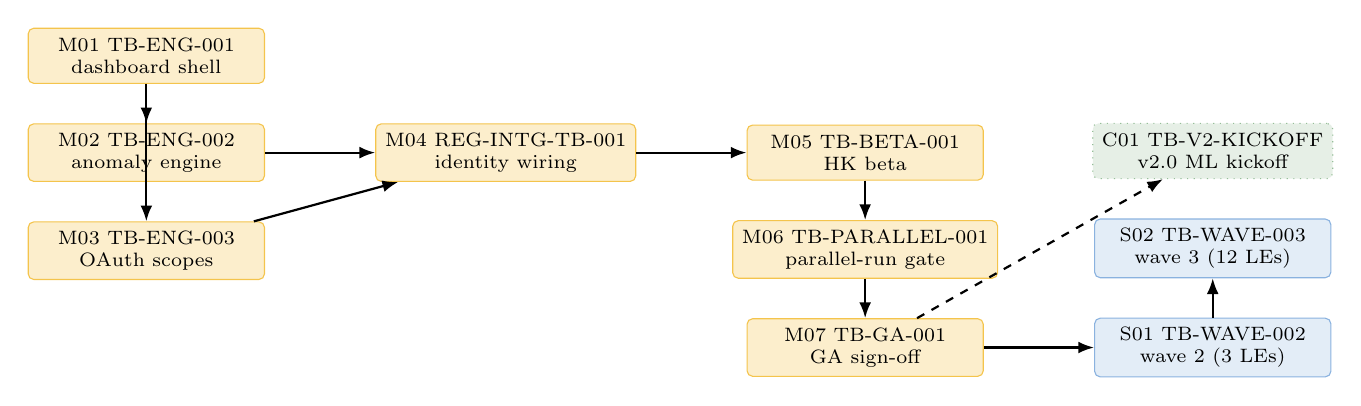
\begin{tikzpicture}[
node distance=5mm and 10mm,
must/.style={draw,rounded corners=2pt,align=center,font=\scriptsize,
fill=tbamber!20,draw=tbamber!70,
minimum height=7mm,minimum width=30mm},
should/.style={draw,rounded corners=2pt,align=center,font=\scriptsize,
fill=tbblue!12,draw=tbblue!50,
minimum height=7mm,minimum width=30mm},
could/.style={draw,rounded corners=2pt,align=center,font=\scriptsize,
fill=tbgreen!12,draw=tbgreen!50,dotted,
minimum height=7mm,minimum width=30mm},
dep/.style={-{Latex[length=2mm]},thick},
soft/.style={-{Latex[length=2mm]},thick,dashed}
]
\node[must] (m01) {M01 TB-ENG-001 \\ \scriptsize dashboard shell};
\node[must,below=of m01] (m02) {M02 TB-ENG-002 \\ \scriptsize anomaly engine};
\node[must,below=of m02] (m03) {M03 TB-ENG-003 \\ \scriptsize OAuth scopes};
\node[must,right=14mm of m02] (m04) {M04 REG-INTG-TB-001 \\ \scriptsize identity wiring};
\node[must,right=14mm of m04] (m05) {M05 TB-BETA-001 \\ \scriptsize HK beta};
\node[must,below=of m05] (m06) {M06 TB-PARALLEL-001 \\ \scriptsize parallel-run gate};
\node[must,below=of m06] (m07) {M07 TB-GA-001 \\ \scriptsize GA sign-off};
\node[should,right=14mm of m07] (s01) {S01 TB-WAVE-002 \\ \scriptsize wave 2 (3 LEs)};
\node[should,above=of s01] (s02) {S02 TB-WAVE-003 \\ \scriptsize wave 3 (12 LEs)};
\node[could,above=of s02] (c01) {C01 TB-V2-KICKOFF \\ \scriptsize v2.0 ML kickoff};

\draw[dep] (m01) -- (m02);
\draw[dep] (m01) -- (m03);
\draw[dep] (m02) -- (m04);
\draw[dep] (m03) -- (m04);
\draw[dep] (m04) -- (m05);
\draw[dep] (m05) -- (m06);
\draw[dep] (m06) -- (m07);
\draw[dep] (m07) -- (s01);
\draw[dep] (s01) -- (s02);
\draw[soft] (m07) -- (c01);
\end{tikzpicture}
\caption{Trial Balance dependency graph. Amber nodes are Must
(critical path); blue are Should (allowance); dotted green are Could
(discretionary). Solid arrows are hard prerequisites; dashed arrows
indicate conditional starts (the target is unlocked when the upstream
completes \emph{and} the v2.0 trigger fires).}
\label{fig:tb-dependency-graph}
\end{figure}

\section{Project milestones}\label{sec:tb-milestones}

\begin{table}[htbp]
\centering
\caption{Trial Balance v1.0 project milestones in dependency order.
Priority: M=Must (critical path), S=Should, C=Could, W=Won't.}
\label{tab:tb-milestones}
\footnotesize
\begin{tabularx}{\linewidth}{@{}l l l l X@{}}
\toprule
\textbf{ID} & \textbf{Prereq} & \textbf{Pri.} & \textbf{Ticket} & \textbf{Milestone} \\ \midrule
M01 & ---       & M & TB-ENG-001         & Dashboard shell in UAT; all 28 workflow states reachable on the HK fixture. \\
M02 & M01       & M & TB-ENG-002         & Statistical anomaly engine passes the fixtures in \cref{ch:controls-engine}. \\
M03 & M01       & M & TB-ENG-003         & OAuth 2.0 scopes enforced end-to-end (\cref{sec:dashboard-api-auth}). \\
M04 & M02, M03  & M & REG-INTG-TB-001    & Identity-attribution wiring (reserve/complete) live in UAT. \\
M05 & M04       & M & TB-BETA-001        & Beta cycle: HK LE only, AI parallel to manual, no business users yet. \\
M06 & M05       & M & TB-PARALLEL-001    & Beta parallel-run gate passes. \\
M07 & M06       & M & TB-GA-001          & GA sign-off by Head of Africa GFS; HK goes live. \\
M08 & M07       & M & TB-BC-REFRESH      & Business-case refresh and compliance attestation (first cycle after GA; then annual). \\
S01 & M07       & S & TB-WAVE-002        & Rollout wave 2: three further LEs onboarded via entity-params (\cref{sec:params-234}). \\
S02 & S01       & S & TB-WAVE-003        & Rollout wave 3: cumulative 12 LEs live. \\
S03 & S02       & S & TB-WAVE-N          & Subsequent waves through full 234-LE coverage (repeated application of the onboarding runbook). \\
C01 & M07 + v2.0 trigger & C & TB-V2-KICKOFF & v2.0 ML anomaly programme kickoff (Chapter~\ref{ch:future-ml}). \\
C02 & M07       & C & TB-COMMENTARY-TUNE & Quarterly commentary-prompt retraining from accept/edit telemetry. \\
W01 & ---       & W & TB-V1-ML           & ML-based anomaly detection is \emph{not} in v1.0 scope (see \cref{ch:future-ml}). \\
W02 & ---       & W & TB-V1-FULL-234     & Full 234-LE rollout is \emph{not} in v1.0 scope; scope for v1.0 ends at wave 3. \\
\bottomrule
\end{tabularx}
\end{table}

\noindent
The Must chain (M01 $\to$ M02/M03 $\to$ M04 $\to$ M05 $\to$ M06 $\to$
M07 $\to$ M08) is the critical path. The Should items (S01--S03) are
the primary \emph{schedule allowance}: if Must items run hot, rollout
waves can slip without affecting v1.0 sign-off. The Could items are
the \emph{scope allowance}: they may be cut to v1.1 without renegotiation.

\section{Launch tiers and exit gates}\label{sec:tb-launch-tiers}

The project walks the four-tier ladder shared across SAP OSS Finance
projects. A tier is exited only when the named exit gate is satisfied;
slippage requires sponsor sign-off.

\begin{table}[htbp]
\centering
\caption{Trial Balance launch tiers. The exit gate defines the MoSCoW
items that must be closed to exit the tier.}
\label{tab:tb-launch-tiers}
\footnotesize
\begin{tabularx}{\linewidth}{@{}l l X@{}}
\toprule
\textbf{Tier} & \textbf{Scope} & \textbf{Exit gate (references MoSCoW IDs)} \\ \midrule
Alpha & Engineering only, DEV + UAT environments, no business users. & M01, M02, M03 closed; all acceptance criteria in \cref{ch:controls} pass on the HK golden fixture; reproducibility of the variance engine confirmed on two consecutive runs. \\
Beta  & One LE (Hong Kong), parallel to the manual process. & M04, M05, M06 closed; parallel-run comparison meets thresholds for one full cycle; no open SEV1/SEV2; audit coverage $=$ 100\,\% of in-scope actions. \\
GA (limited) & Three LEs (HK plus wave 2). & M07 closed; Beta gate sustained for two consecutive cycles; S01 closed; entity-params onboarding runbook exercised end-to-end; kill-switch green. \\
Full rollout & All LEs in scope for v1.0 (through wave 3). & S02 closed; two quarterly reviews sustained; M08 complete; business-case refresh complete; EUC retirement plan (\cref{sec:euc-retirement-plan}) at ``dashboard authoritative'' for all three EUCs. \\
\bottomrule
\end{tabularx}
\end{table}

\section{Kill-switch conditions}\label{sec:tb-kill-switch}

The kill-switch is a pre-committed rulebook: a tripped condition enters
the action column without further debate. GFAIC and sponsor are
notified within 24 hours. The conditions are evaluated continuously
(on every cycle) and do not carry dates.

\begin{table}[htbp]
\centering
\caption{Trial Balance kill-switch.}
\label{tab:tb-kill-switch}
\footnotesize
\begin{tabularx}{\linewidth}{@{}l l X@{}}
\toprule
\textbf{Condition} & \textbf{Evaluation} & \textbf{Action} \\ \midrule
Parallel-run disagreement rate $>$\,10\,\% on three consecutive cycles & per cycle & \textbf{Abandon v1.0}; fall back to manual; re-scope v1.1. \\
Cycle time from \stateid{EXTRACT\_TB} to \stateid{SEND\_FORTM} $>$\,manual baseline for two cycles & per cycle & \textbf{Redesign}: halt rollout, fix latency, re-enter Beta. \\
Accept-without-edit rate of AI commentary $<$\,40\,\% for two cycles & per cycle & \textbf{Redesign prompt layer}; commentary drafts gated behind a feature flag. \\
Audit-coverage gap (missed \texttt{reserve/complete} pair) detected in production & continuous & \textbf{Pause GA onboarding}; incident-review before next wave. \\
Any MAS MGF finding attributable to TB specifically & continuous & \textbf{Halt rollout}; remediate before next wave. \\
Shared-platform dependency in \cref{tab:tb-shared-deps} declared red by its owner project & continuous & \textbf{Pause downstream Must}; re-plan at next steering. \\
\bottomrule
\end{tabularx}
\end{table}

\section{Shared-platform dependencies}\label{sec:tb-shared-deps}

This project depends on four shared-platform components. Each is owned
by a sibling project (Regulations) or by shared infra, and is tracked
here only as a dependency, not a commitment this project can
unilaterally adjust. Sequence is expressed in terms of the Must item
that first consumes the dependency, not in calendar time.

\begin{table}[htbp]
\centering
\caption{Shared-platform dependencies.}
\label{tab:tb-shared-deps}
\footnotesize
\begin{tabularx}{\linewidth}{@{}l l l X@{}}
\toprule
\textbf{Component} & \textbf{Owner} & \textbf{First consumed by} & \textbf{Impact if late} \\ \midrule
Audit service (reserve/complete, immutable storage) & Regulations project & M04 (REG-INTG-TB-001) & No Beta gate possible without this; TB GA slips in lockstep with the audit service. \\
Unified schema registry (\path{docs/schema/}) & Shared infra & M01 & Already \texttt{migration.status=complete}; no remaining risk. \\
vLLM hosting (\texttt{vllm-only} policy) & Shared platform & M02 & Graceful-degradation ladder defined in the Regulations spec provides fallback; slip tolerable. \\
Review dashboard infra (SAPUI5 + BTP destination) & Shared platform & M01 & Degrade to read-only evidence mirror on Shared Drive; EUC retirement timeline reopens. \\
\bottomrule
\end{tabularx}
\end{table}

\noindent
Shared-platform dependencies are surfaced at monthly steering. If any
upstream owner declares \textbf{amber} or \textbf{red} on a component
in \cref{tab:tb-shared-deps}, the affected downstream Must milestone
is re-planned at the following steering.

\section{Governance and business-case cadence}\label{sec:tb-governance}

\paragraph{Project governance.}
The Trial Balance project reports monthly to a project steering
(Process Owner, Head of Africa GFS, AI Engineer) and quarterly to the
cross-project GFAIC (\cref{ch:controls}). Monthly steering accepts or
rejects amber/red signals on Must items; GFAIC reviews compliance
posture and any cross-project dependencies.

\paragraph{Business-case refresh (M08).}
The 2025-12-14 business case that authorises this project is refreshed
on the following rhythm:

\begin{itemize}
\item \textbf{Mandatory refresh}: at the first cycle after GA, and
annually thereafter (ticket TB-BC-REFRESH, priority M in
\cref{tab:tb-milestones}). Refresh packet includes volume
assumptions, unit economics,
FTE leverage realised vs.\ forecast, and a deviation statement
against the 2025-12-14 baseline.
\item \textbf{Trigger-based refresh}: any of
\begin{itemize}
\item LE count in scope changes by $\ge\,20$\,\% from forecast
(either direction);
\item per-cycle run cost changes by $\ge\,30$\,\% (vLLM
licensing, GPU price, variance-engine throughput);
\item new regulatory obligation materially affecting scope
(e.g.\ new MAS MGF pillar, additional jurisdiction);
\item any kill-switch in \cref{tab:tb-kill-switch} is tripped.
\end{itemize}
\item \textbf{Owner}: business sponsor (TB-REQ-001 author,
S.~Badrinath, or delegate). Approval routed through the
project steering and filed at
\path{docs/tb/business-case/refresh-history.yaml}.
\end{itemize}
\chapter{Agent Implementation Instructions}\label{ch:agent-impl}

\section{Purpose and audience}
This chapter is the self-contained, intent-based instruction set for
implementing the \emph{Trial Balance review} domain inside the
unified SAP OSS platform. It is written for LLM-driven and human
implementation agents who will extend existing services to realise
the specification. It assumes only this PDF; every platform
decision, integration contract, and governance obligation the TB
workstream depends on is restated here so that no companion document
is required. Existing chapters~\ref{ch:overview}--\ref{ch:tb-roadmap}
remain the normative source for the TB domain itself; this chapter
tells future agents \emph{how} to build what those chapters
describe, \emph{where} to put it in the codebase, and \emph{how} it
plugs into the wider platform.

% !TEX root = ../master.tex
% =============================================================================
% MASTER PLATFORM CORE: Shared Intent-Based Instructions (Union)
% World-Class Version: HITL Gates, Process Integrity, and .clinerules Wiring
% =============================================================================

\section{Rules of Engagement for AI Agents}
\label{sec:agent-rules}

To ensure safety and architectural integrity, all implementation agents must adhere to the following Prime Directives:

\begin{enumerate}[label=\textsc{rule}-\arabic*:, leftmargin=2cm]
\item \textbf{Credential Protection.} Never log, print, or commit secrets. Use the \texttt{.secrets.example} pattern for all new integrations.
\item \textbf{Context Efficiency.} Prioritize surgical edits. Request only the minimum required file ranges to satisfy the task intent.
\item \textbf{Test-Driven Implementation.} No code is complete without a corresponding fixture in \texttt{tests/fixtures/} and a passing validation run.
\item \textbf{Self-Correction.} If a schema validation fails, the agent must diagnose the root cause (hallucination vs. schema drift) before re-attempting implementation.
\item \textbf{Safety Inheritance.} Domain-specific agent rules (\texttt{.clinerules}) may only \emph{tighten} (e.g., lower timeout, stricter precision), never \emph{loosen} regulatory constraints.
\end{enumerate}

\section{Agent Rule-Pack Architecture (.clinerules)}
\label{sec:agent-rule-packs}

The platform mandates a three-tier inheritance hierarchy for agent behavior. Implementation agents must load the relevant rule pack before starting any task.

\subsection{Inheritance Hierarchy}
\begin{enumerate}
\item \textbf{Repository-level (\texttt{/.clinerules}):} The baseline for all engineering and documentation standards.
\item \textbf{Intelligence-level (\texttt{/src/intelligence/.clinerules}):} The regulatory envelope (MAS MGF) that wraps all domains.
\item \textbf{Domain-level (\texttt{/src/<domain>/.clinerules}):} Domain-specific constraints (e.g., Arabic character precision).
\end{enumerate}

\subsection{Safety-Critical Flags}
The following flags in the rule packs are subject to \textsc{rule-5} (Inherit, Never Weaken):
\begin{table}[htbp]
\centering
\footnotesize
\caption{Safety-Critical Agent Flags.}
\label{tab:safety-flags}
\begin{tabularx}{\textwidth}{@{}l X X@{}}
\toprule
\textbf{Flag} & \textbf{Parent Value (Regs)} & \textbf{Tightening Direction} \\
\midrule
\texttt{deny\_by\_default} & \texttt{true} & Invariant (Cannot be set to false). \\
\texttt{require\_identity} & \texttt{true} & Invariant (Cannot be bypassed). \\
\texttt{max\_retries} & \texttt{3} & May only \emph{decrease}. \\
\texttt{timeout\_ms} & \texttt{30000} & May only \emph{decrease}. \\
\bottomrule
\end{tabularx}
\end{table}

\section{Platform Overview --- One Codebase, One Instance}
\label{sec:agent-platform-overview}

\subsection{Integration Stance}
The SAP OSS platform is delivered as a single codebase that runs as a single logical instance. All cross-cutting concerns are hosted by existing services.

\begin{adrbox}{{One Codebase, One Instance}}
To minimize integration latency and eliminate distributed-system failure modes (e.g., partial partitions), we mandate a single logical instance. All cross-domain orchestration happens via the MCP Gateway layer.
\end{adrbox}

\subsection{Platform Integration Map}
\label{sec:platform-map}

\begin{figure}[htbp]
\centering
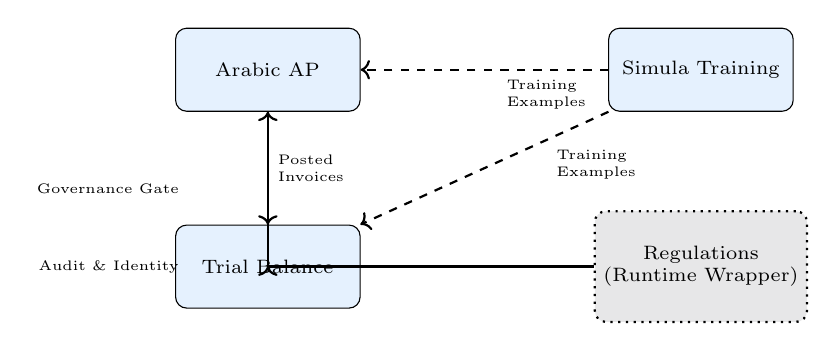
\begin{tikzpicture}[
node distance=2.5cm,
auto,
block/.style={rectangle, draw, rounded corners, fill=sapblue!10, text width=6em, text centered, minimum height=3em, font=\scriptsize},
regs/.style={rectangle, draw, rounded corners, fill=sapgrey!20, text width=7em, text centered, minimum height=4em, thick, dotted, font=\scriptsize}
]
\node (arabic) [block] {Arabic AP};
\node (tb) [block, below of=arabic] {Trial Balance};
\node (simula) [block, right of=arabic, node distance=5.5cm] {Simula Training};
\node (regs) [regs, below of=simula] {Regulations (Runtime Wrapper)};

\draw [->, thick] (arabic) -- node [align=left, font=\tiny] {Posted\\Invoices} (tb);
\draw [->, thick, dashed] (simula) -- node [align=left, font=\tiny, near start] {Training\\Examples} (arabic);
\draw [->, thick, dashed] (simula) -- node [align=left, font=\tiny, near start] {Training\\Examples} (tb);
\draw [->, thick] (regs) -| node [font=\tiny, near end, xshift=-1cm] {Governance Gate} (arabic);
\draw [->, thick] (regs) -| node [font=\tiny, near end, xshift=-1cm] {Audit \& Identity} (tb);
\end{tikzpicture}
\caption{Cross-domain interaction and unified data flow map. Detailed governance logic is defined in \cref{reg:ch:mgf}.}
\end{figure}

\section{Transactional Sequence Diagrams}
\label{sec:agent-sequences}

Implementation agents must adhere to the temporal logic defined below. Every cross-domain request MUST be brokered by the Regulations Wrapper.

\subsection{Universal Governance Handshake}
This sequence applies to \textbf{all} platform service calls.

\begin{figure}[htbp]
\centering
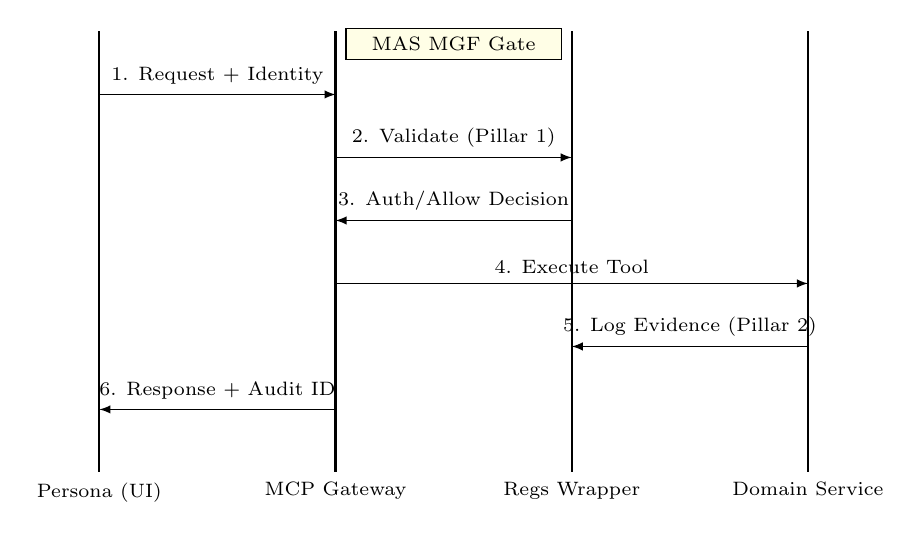
\begin{tikzpicture}[x=1cm, y=-0.8cm, font=\scriptsize]
% Lifelines
\draw[thick] (0,0) -- (0,7) node[below] {Persona (UI)};
\draw[thick] (3,0) -- (3,7) node[below] {MCP Gateway};
\draw[thick] (6,0) -- (6,7) node[below] {Regs Wrapper};
\draw[thick] (9,0) -- (9,7) node[below] {Domain Service};

% Interaction
\draw[->, >=latex] (0,1) -- node[above] {1. Request + Identity} (3,1);
\draw[->, >=latex] (3,2) -- node[above] {2. Validate (Pillar 1)} (6,2);
\draw[<-, >=latex] (3,3) -- node[above] {3. Auth/Allow Decision} (6,3);
\draw[->, >=latex] (3,4) -- node[above] {4. Execute Tool} (9,4);
\draw[->, >=latex] (9,5) -- node[above] {5. Log Evidence (Pillar 2)} (6,5);
\draw[<-, >=latex] (0,6) -- node[above] {6. Response + Audit ID} (3,6);

\node[draw, fill=yellow!10, text width=2.5cm, align=center] at (4.5,0.2) {MAS MGF Gate};
\end{tikzpicture}
\caption{Standard platform handshake for governed tool execution. Audit schemas are detailed in \cref{reg:ch:identity}.}
\end{figure}

\subsection{Arabic AP Golden Path}
Temporal flow for invoice processing with Arabic context.

\begin{figure}[htbp]
\centering
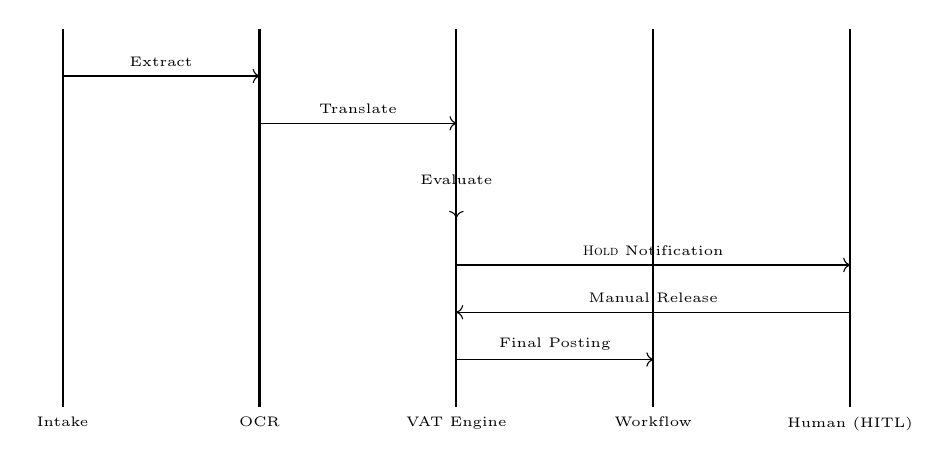
\begin{tikzpicture}[x=1cm, y=-0.6cm, font=\tiny]
\draw[thick] (0,0) -- (0,8) node[below] {Intake};
\draw[thick] (2.5,0) -- (2.5,8) node[below] {OCR};
\draw[thick] (5,0) -- (5,8) node[below] {VAT Engine};
\draw[thick] (7.5,0) -- (7.5,8) node[below] {Workflow};
\draw[thick] (10,0) -- (10,8) node[below] {Human (HITL)};

\draw[->] (0,1) -- node[above] {Extract} (2.5,1);
\draw[->] (2.5,2) -- node[above] {Translate} (5,2);
\draw[->] (5,3) -- node[above] {Evaluate} (5,4); % Internal loop
\draw[->] (5,5) -- node[above] {\textsc{Hold} Notification} (10,5);
\draw[<-] (5,6) -- node[above] {Manual Release} (10,6);
\draw[->] (5,7) -- node[above] {Final Posting} (7.5,7);
\end{tikzpicture}
\caption{Arabic AP sequence: Scanned PDF to Release. VAT rules are specified in \cref{ar:ch:vat}.}
\end{figure}

\section{Compute and Resource Alignment}
\label{sec:hardware-profiles}

AI algorithms are calibrated for the reference infrastructure established in the domain chapters:

\begin{table}[htbp]
\centering
\footnotesize
\caption{Infrastructure Reference Profiles.}
\label{tab:hardware-profiles}
\begin{tabularx}{\textwidth}{@{}l X X@{}}
\toprule
\textbf{Workload} & \textbf{Reference Hardware} & \textbf{Performance Target} \\
\midrule
LLM Inference & NVIDIA L40S (48GB) & AWQ 4-bit / p95 < 2s \\
Embeddings & NVIDIA A100 (40/80GB) & FP16 / p99 < 500ms \\
Simula Training & NVIDIA A100 SXM4 cluster & BF16 throughput parity \\
\bottomrule
\end{tabularx}
\end{table}

\section{Human-in-the-Loop (HITL) Critical Gates}
\label{sec:hitl-gates}

The following "Four-Eyes" gates are mandatory. AI agents must implement the "Awaiting Sign-off" state for these actions:
\begin{itemize}
\item \textbf{VAT Release:} No invoice marked as \textsc{hold} can be released without human review (see \cref{ar:ch:ap}).
\item \textbf{Anomaly Override:} Statistical outliers ($3\sigma$) cannot be dismissed by AI; only "Confirmed" or "Triaged" by human (see \cref{tb:ch:controls}).
\item \textbf{Journal Posting:} Agents may \emph{draft} journal entries, but only the Financial Controller persona can \emph{commit} to S/4HANA (see \cref{tb:ch:controls-engine}).
\end{itemize}

\section{Registry Integrity \& Live Status}
\label{sec:registry-integrity}

Before initiating any schema-dependent task, implementation agents must verify the live status of the Unified Schema Registry (see \cref{sim:chap:schema}).
\begin{adrbox}{Registry First}
If \texttt{docs/schema/registry.json} is out of sync with the codebase, the agent must halt and emit a \textsc{schema-mismatch} event.
\end{adrbox}

\section{Master Implementation Manifest (Union)}
Implementation runs in three waves across the entire platform.

\subsection*{Wave 1 --- Foundations}
\begin{itemize}
\item \textbf{Simula:} Implement HANA schema extraction pipeline (MCP discovery). See \cref{sim:chap:extraction}.
\item \textbf{Regulations:} Implement MAS MGF Pillar 1 logic (Tool allow-list). See \cref{reg:ch:mgf}.
\item \textbf{Arabic:} Implement Invoice Intake \& OCR Gateway. See \cref{ar:ch:ai}.
\item \textbf{Trial Balance:} Implement identity-attribution wiring. See \cref{reg:ch:identity}.
\end{itemize}

\subsection*{Wave 2 --- Core Domain Build-out}
\begin{itemize}
\item \textbf{Trial Balance:} Implement Controls \& Commentary Engine (3$\sigma$ anomaly logic). See \cref{tb:ch:ai,tb:ch:controls-engine}.
\item \textbf{Arabic:} Implement multi-country VAT Engine (Saudi, UAE, Bahrain, Oman). See \cref{ar:ch:vat,ar:ch:vat-impl}.
\item \textbf{Simula:} Implement Taxonomy Generation \& Agentic Data Synthesis. See \cref{sim:chap:taxonomy,sim:chap:generator}.
\item \textbf{Trial Balance:} Realise 28-state BPMN workflow (\texttt{tb-review-glo}). See \cref{tb:ch:workflow}.
\end{itemize}

\subsection*{Wave 3 --- Hardening}
\begin{itemize}
\item \textbf{Regulations:} Implement Per-Request Identity Attribution. See \cref{reg:ch:identity}.
\item \textbf{Trial Balance:} Deliver Human Review Dashboard. See \cref{tb:ch:review-dashboard}.
\item \textbf{Simula:} Deliver test fixtures and testing at 85\% coverage. See \cref{sim:ch:test-fixtures,sim:ch:testing}.
\item \textbf{Regulations:} Wire Emergent-Capability monitoring. See \cref{reg:ch:monitoring}.
\end{itemize}

\section{Governance Obligations (MAS MGF)}
The regulations domain wraps all service calls at runtime. Agents must implement the following hooks in every domain:
\begin{itemize}
\item \textbf{Pillar 1:} Tool allow-list enforcement (deny-by-default).
\item \textbf{Pillar 2:} Traceability via the identity attribution envelope.
\item \textbf{Pillar 3:} Metric emission to the monitoring sink.
\end{itemize}
Detailed pillar requirements are defined in \cref{reg:ch:mgf}.

\section{FMEA: Failure Mode and Effects Analysis for AI}
\label{sec:fmea-ai}

The following analysis identifies critical AI failure modes within the TB pipeline and their deterministic mitigations.

\begin{table}[htbp]
\centering
\footnotesize
\caption{FMEA for Trial Balance AI Pipeline.}
\label{tab:tb-fmea}
\begin{tabularx}{\textwidth}{@{}l X X X@{}}
\toprule
\textbf{Failure Mode} & \textbf{Symptom} & \textbf{Impact} & \textbf{Technical Mitigation} \\
\midrule
LLM Hallucination & Commentary references accounts not in the input TB. & High (Inaccuracy) & Cross-check extracted accounts against the input TB record. \\
Normality Drift & $3\sigma$ fails due to non-normal variance distribution. & Medium (False Neg.) & Fallback to MAD (Median Absolute Deviation) scoring. \\
Prompt Injection & Malicious input triggers unverified journal posting. & Critical (Security) & Deterministic rule-check gate on all POST endpoints. \\
\bottomrule
\end{tabularx}
\end{table}

\section{This domain in context}
\label{sec:agent-domain-context}
Trial Balance review is the finance close workstream among the four
domains. Its primary persona is the Financial Controller, whose
working view is the review dashboard surfaced through the shared
workspace shell and gated by TB entitlements. The domain's entry
points are the TB extract feed and the upstream AP postings
(including those produced by the Arabic domain); its exit points are
(a)~signed-off commentary records, (b)~evidenced controls for the
month-end close, and (c)~any journal corrections posted back to SAP
S/4HANA. Every artefact is validated against the TB-owned schemas in
\texttt{structured/schema/} before it leaves the service. The domain
depends on the horizontal regulations wrapper for runtime governance
and on Simula for the training corpus used by the anomaly-detection
and commentary models described in chapter~\ref{ch:ai}.

\section{Schema contribution}
\label{sec:agent-schema-contrib}
TB owns the schemas catalogued in chapter~\ref{ch:schema} and listed
in~\ref{tab:schemas}. The canonical set is the control record
(\S\ref{sec:control-schema}, fields in~\ref{tab:control-fields}), the
decision-point record (\S\ref{sec:decision-point-schema}), the
workflow record (\S\ref{sec:workflow-schema},
header fields in~\ref{tab:workflow-fields}), and TB's own
\texttt{requirement.schema.json}. These schemas live under
\texttt{docs/latex/specs/tb/} as normative text and under
\texttt{structured/schema/} as the JSON Schema artefacts consumed at
runtime. Registration in the unified registry is additive: each
schema is listed in
\texttt{src/intelligence/ai-core-pal/data\_products/registry.yaml}
with its URI, owning domain (\texttt{tb}), security class
(\texttt{confidential}), and LLM routing (\texttt{vllm-only}),
following the ODPS~4.1 pattern. Simula consumes these schemas
directly as inputs to its extraction pipeline; it does not transform
them. TB's \texttt{requirement.schema.json} is a distinct URI from
regulations' \texttt{requirement.schema.json}; the two files are not
merged.

\section{Persona and MCP allow-list}
\label{sec:agent-persona}
\begin{itemize}
\item \textbf{Persona id:} \texttt{financial-controller}.
\item \textbf{Roles:} TB ingestion and validation, anomaly triage,
commentary drafting and review, control evidencing, close
sign-off.
\item \textbf{Entitlements:} read/write on the TB control record,
decision-point record, and workflow record; advance transitions
on the 28 states of \texttt{tb-review-glo}
(chapter~\ref{ch:workflow},~\ref{tab:states}); evidence-write on
the control enforcement map in~\ref{fig:controls-map}; journal
posting on corrected entries (chapter~\ref{ch:controls-engine}).
\item \textbf{UI route:} \texttt{/tb/\{tenant\}/review} on the
shared workspace shell; surfaced only to callers whose
entitlement set includes \texttt{financial-controller}.
\item \textbf{MCP tool allow-list:}
\texttt{tb.ingest}, \texttt{tb.anomaly.detect},
\texttt{tb.commentary.draft}, \texttt{tb.commentary.validate},
\texttt{tb.workflow.advance}, \texttt{tb.control.evidence},
\texttt{tb.journal.post}. All other MCP tools are denied by
default per MAS MGF pillar~1.
\end{itemize}

\section{Agent Rule-Pack Binding}
\label{sec:agent-rule-binding}
Before initiating any task in this domain, the agent MUST load the following rule packs in order:
\begin{enumerate}
\item \filepath{.clinerules} (Global Standards)
\item \filepath{src/intelligence/.clinerules} (Regulations Envelope)
\item \filepath{src/tb/.clinerules} (TB Domain Constraints)
\end{enumerate}

\section{Implementation tasks for this domain}
\label{sec:agent-tasks}
The tasks below are intent-based: each task states the outcome a
future agent must achieve and the location in the existing codebase
where the work belongs. None of them contains code; each task binds
to the TB chapters that define the required behaviour.

\subsection*{Task T1 --- Controls and commentary engine}
\textbf{Intent.} Implement the controls and commentary engine
specified in chapter~\ref{ch:controls-engine}, including the decision
tree (\ref{fig:decision-tree}), the rule format, materiality
thresholds, and journal posting.

\begin{adrbox}{Why 3-Sigma?}
We chose $3\sigma$ for v1.0 to ensure immediate baseline stability. This statistical floor provides a 99.7\% confidence interval for known variance patterns while the ML training set accumulates.
\end{adrbox}

\textbf{In-scope.} Per-rule evaluators for the anomaly checks in
~\ref{tab:anomalies} (3$\sigma$, MAD, percentile); materiality-aware
commentary generation; deadline-aware investigation routing.
\textbf{Out-of-scope.} The v2.0 ML-based anomaly detection explored
in chapter~\ref{ch:future-ml}; that work is reserved for a later
release and must remain behind a feature flag.
\textbf{Paths to extend.} AI pipeline stages in
chapter~\ref{ch:ai}, specifically stage~2 (anomaly detection) and
stage~3 (commentary drafting); engine module colocated with the
gateway service.
\textbf{Definition of done.} Every anomaly check
in~\ref{tab:anomalies} has a callable rule; commentary draft records
validate against the TB schema set and carry the evidencing required
by chapter~\ref{ch:controls-engine}.

\textbf{Autonomous Verification (Agent Logic):}
\begin{lstlisting}[language=jsonx]
// Verify Task T1
{
"test_fixture": "tests/fixtures/tb/golden_sample.json",
"expected_outcome": "anomaly_count == 5",
"validation_command": "pytest src/tb/engine_test.py --verify-rules"
}
\end{lstlisting}

\textbf{Verification.} Unit tests for each rule pass; the commentary
draft endpoint produces records that pass validation.

\subsection*{Task T2 --- 28-state BPMN workflow}
\textbf{Intent.} Realise the \texttt{tb-review-glo} workflow in
chapter~\ref{ch:workflow}, including all 28 states
in~\ref{tab:states} and the preparation
(\ref{fig:prep-phase}), analysis (\ref{fig:analysis-phase}), and
sign-off phases.
\textbf{In-scope.} State transitions, phase gates, deadline handling,
roll-back and park semantics.
\textbf{Out-of-scope.} BPMN-driven cross-tenant orchestration; the
workflow runs within a single tenant per instance.
\textbf{Paths to extend.} Workflow engine hosted in the gateway
service; workflow record defined in chapter~\ref{ch:schema}.
\textbf{Definition of done.} All 28 states are reachable from a
deterministic predecessor; every transition is audit-logged with the
persona id; rolling the golden sample through the workflow produces
the signed-off close artefact without manual intervention.
\textbf{Verification.} Workflow unit tests pass; the review-dashboard
chapter (\ref{ch:review-dashboard}) queue view surfaces the expected
filter counts.

\subsection*{Task T3 --- Review dashboard}
\textbf{Intent.} Deliver the human review dashboard specified in
chapter~\ref{ch:review-dashboard}.
\textbf{In-scope.} Queue view with the fields in~\ref{tab:queue-fields},
sorting/filtering, bulk operations, review view, commentary
composition aids, sign-off flow.
\textbf{Out-of-scope.} Mobile layouts; cross-period comparative
analytics beyond what chapter~\ref{ch:review-dashboard} lists.
\textbf{Paths to extend.} Persona surface within
\texttt{generativeUI/training-webcomponents-ngx}; data-fetching
hooks that call the TB MCP tools enumerated above.
\textbf{Definition of done.} The dashboard renders the queue view,
supports the bulk operations listed in the chapter, and writes
control-evidence records through the allow-listed MCP tools.
\textbf{Verification.} Dashboard component tests pass; the persona
entitlement gate returns 403 for non-Financial-Controller callers.

\subsection*{Task T4 --- Controls and acceptance}
\textbf{Intent.} Wire the control enforcement map and acceptance
criteria in chapter~\ref{ch:controls}, including the EUC evidencing
requirement in~\ref{sec:controls-eucs}.
\textbf{In-scope.} Control-to-state binding per~\ref{fig:controls-map};
risk register mitigations from~\ref{tab:risks}; EUC evidencing hooks.
\textbf{Out-of-scope.} External SOX reporting system integration.
\textbf{Paths to extend.} Control catalogue file referenced in
chapter~\ref{ch:controls}; evidence store.
\textbf{Definition of done.} Every control fires on its bound
states; evidence records are produced; the acceptance criteria
checklist in chapter~\ref{ch:controls} is satisfied.
\textbf{Verification.} Running the TB golden sample triggers every
control; the evidence report reconciles with the acceptance
checklist.

\subsection*{Task T5 --- Testing and coverage}
\textbf{Intent.} Deliver the testing specification in
chapter~\ref{ch:testing} at the coverage thresholds
in~\ref{tab:tb-coverage}.
\textbf{In-scope.} TB extract fixtures, variance fixtures, unit
tests for variance detection and commentary drafting, integration
tests through the workflow, regression fixtures.
\textbf{Out-of-scope.} Load and performance benchmarking beyond what
chapter~\ref{ch:testing} defines.
\textbf{Paths to extend.} Test directory colocated with the TB
service code; fixture store used by Simula as training input.
\textbf{Definition of done.} Coverage meets the thresholds
in~\ref{tab:tb-coverage}; CI gates block regressions.
\textbf{Verification.} \texttt{make spec-tb} remains green; the TB
test entry points listed in chapter~\ref{ch:testing} all run.


\section{Governance obligations applied to this domain}
\label{sec:agent-governance}
The regulations domain wraps Trial Balance review at runtime. Four
obligations apply without exception; each is stated as a concrete
hook in the TB codebase.

\begin{itemize}
\item \textbf{MAS MGF four pillars} (see regulations
chapter~3 in
\texttt{docs/latex/specs/regulations/chapters/03-mgf-framework.tex}).
Pillar~1 (assess and bound): every TB MCP tool is declared in the
allow-list in \S\ref{sec:agent-persona}, deny-by-default.
Pillar~2 (design and deploy): the pipeline stages in
chapter~\ref{ch:ai} are traceable end-to-end via the per-request
identity attribution described below. Pillar~3 (operate and
monitor) and pillar~4 (govern and disclose) are satisfied by
emitting the evidence records produced by the TB control
catalogue (chapter~\ref{ch:controls}) into the shared governance
store.
\item \textbf{Identity attribution} (regulations chapter~10,
\texttt{10-identity-attribution.tex}). Every MCP call and every
workflow transition carries the persona id, agent id, request id,
and tenant id. The gateway is the attachment point; TB code
propagates the identity envelope without mutating it.
\item \textbf{Emergent-capability monitoring} (regulations
chapter~8, \texttt{08-monitoring-spec.tex}). Anomaly detection,
commentary drafting, and workflow state transitions are
instrumented with the monitoring metrics specified in that
chapter; metrics flow to the monitoring sink defined there.
\item \textbf{Conformance tooling} (regulations chapter~6,
\texttt{06-conformance-tooling.tex}). The TB service exposes
AI Verify 2.0 plug-in hooks and Moonshot CI/CD 1.1.0 benchmark
entry points as required by that chapter.
\end{itemize}

\section{Cross-spec integration --- full detail}
\label{sec:agent-integration}

\subsection{With Arabic AP}
Arabic AP produces posted AP records and VAT checklists that feed
the TB close. TB consumes them as evidence inputs to its commentary
engine, not as schema merges: the Arabic invoice schema and the TB
control record remain distinct URIs in the unified registry.
Integration point: TB's ingestion stage calls the Arabic MCP tool
\texttt{invoice.extract-fields} with read-only entitlements; the
response is validated against \texttt{invoice.schema.json} before TB
accepts it.

\subsection{With Trial Balance}
TB exports the control record, decision-point record, workflow
record, and its own \texttt{requirement.schema.json} under
\texttt{structured/schema/} (chapter~\ref{ch:schema}); registers the
MCP tools enumerated in \S\ref{sec:agent-persona}; and applies the
four governance hooks in \S\ref{sec:agent-governance} to every call
it serves. External consumers (Arabic, regulations, Simula) see TB
only through these contracts; there are no private back-channels.

\subsection{With Regulations}
Regulations wraps TB at runtime. Every TB MCP call is brokered
through the regulations governance gate, which applies pillars~1--4
of MAS MGF, attaches the identity envelope, and routes
emergent-capability metrics to the monitoring store. The TB service
code does not call regulations directly; the gateway layer enforces
this. Conformance tests defined in regulations chapter~5 (empirical
evidence) and chapter~6 (conformance tooling) execute against the TB
service as part of the platform CI gate.

\subsection{With Simula}
Simula consumes TB's schemas and fixtures as training input. The
contract is schema-in, \texttt{TrainingExample}-out: Simula reads the
TB schema set and the TB fixture store; it produces
\texttt{TrainingExample} records. Simula does not call TB MCP tools
at runtime and does not share state with the TB workflow. No
cross-domain operational envelope is introduced.

\section{Wave assignment and sequencing}
\label{sec:agent-waves}
Implementation runs in three waves.

\begin{itemize}
\item \textbf{Wave 1 --- foundations.} Unified schema registry
entry; persona-gated surface for the Financial Controller;
identity attribution envelope flowing through the gateway.
Prerequisites: the regulations chapter~10 identity schema must
be frozen.
\item \textbf{Wave 2 --- TB core build-out.} Tasks T1, T2, T3, T4
above. Prerequisites: Wave~1 complete; Simula training fixtures
available from Simula Wave~1 (extraction pipeline); Arabic MCP
tool \texttt{invoice.extract-fields} reachable.
\item \textbf{Wave 3 --- hardening and conformance.} Task T5 and
full conformance-tooling hook-up. Prerequisites: Wave~2 complete;
regulations Wave~2 conformance tooling integrated; monitoring
sink live.
\end{itemize}

TB occupies Wave~2 for its core build-out and Wave~3 for its testing
and conformance surfaces.

\section{Acceptance criteria (platform-wide)}
\label{sec:agent-acceptance}
When all four chapter~12 instruction sets are implemented, the
platform satisfies the following invariants:

\begin{enumerate}
\item \textbf{One instance.} A single codebase runs a single
logical instance; no domain ships as a separate product.
\item \textbf{Persona-gated surfaces.} The four personas each
reach a tailored UI on the shared shell; no route, MCP tool, or
data product is visible outside its persona's entitlement set.
\item \textbf{Unified registry.} Every schema in use is listed in
the ODPS~4.1 registry under its owning domain; validators
resolve \texttt{\$ref}s through the unified registry only.
\item \textbf{No schema merges.} The two
\texttt{requirement.schema.json} files in TB and regulations
remain distinct; no cross-domain composite schemas are produced.
\item \textbf{No cross-domain operational envelope.} Runtime
orchestration stays within each domain's service; only Simula
consumes other domains' outputs, and only as training input.
\item \textbf{Governance wraps all three non-regulations domains.}
Arabic, TB, and Simula service calls pass through the
regulations runtime wrapper without exception.
\end{enumerate}

\section{References}
\label{sec:agent-references}
Within-spec references:
chapter~\ref{ch:overview} (overview),
chapter~\ref{ch:schema} (data schema),
chapter~\ref{ch:ai} (AI augmentation pipeline),
chapter~\ref{ch:controls-engine} (controls and commentary engine),
chapter~\ref{ch:workflow} (workflow and approval engine),
chapter~\ref{ch:controls} (controls, testing and acceptance),
chapter~\ref{ch:references} (references),
chapter~\ref{ch:review-dashboard} (review dashboard),
chapter~\ref{ch:testing} (testing specification),
chapter~\ref{ch:future-ml} (future ML work),
chapter~\ref{ch:tb-roadmap} (project roadmap).

Peer chapter~12 instruction sets for the other three domains (each
is self-contained; consult directly when operating in that domain):
\begin{itemize}
\item Arabic AP:
\texttt{docs/latex/specs/arabic/chapters/12-implementation-instructions.tex}.
\item Regulations:
\texttt{docs/latex/specs/regulations/chapters/12-implementation-instructions.tex}.
\item Simula:
\texttt{docs/latex/specs/simula/chapters/12-implementation-instructions.tex}.
\end{itemize}

Shared platform artefacts:
\begin{itemize}
\item ODPS~4.1 registry:
\texttt{src/intelligence/ai-core-pal/data\_products/registry.yaml}.
\item Schema pipeline and resolver:
\texttt{src/intelligence/schema\_pipeline/}.
\item Training pipeline (Simula):
\texttt{src/training/pipeline/}.
\item Shared workspace shell:
\texttt{generativeUI/training-webcomponents-ngx}.
\end{itemize}

% --- Incorporated Universal Chapters ---
\chapter{Global Wave-Dependency Manifest}
\label{ch:global-dependencies}

\section{Critical Path Visualization (Waves 1--3)}
The following chart defines the normative sequencing for implementation agents. A task in a later wave cannot be marked \textsc{complete} until its prerequisites in an earlier wave are validated.

\begin{figure}[htbp]
\centering
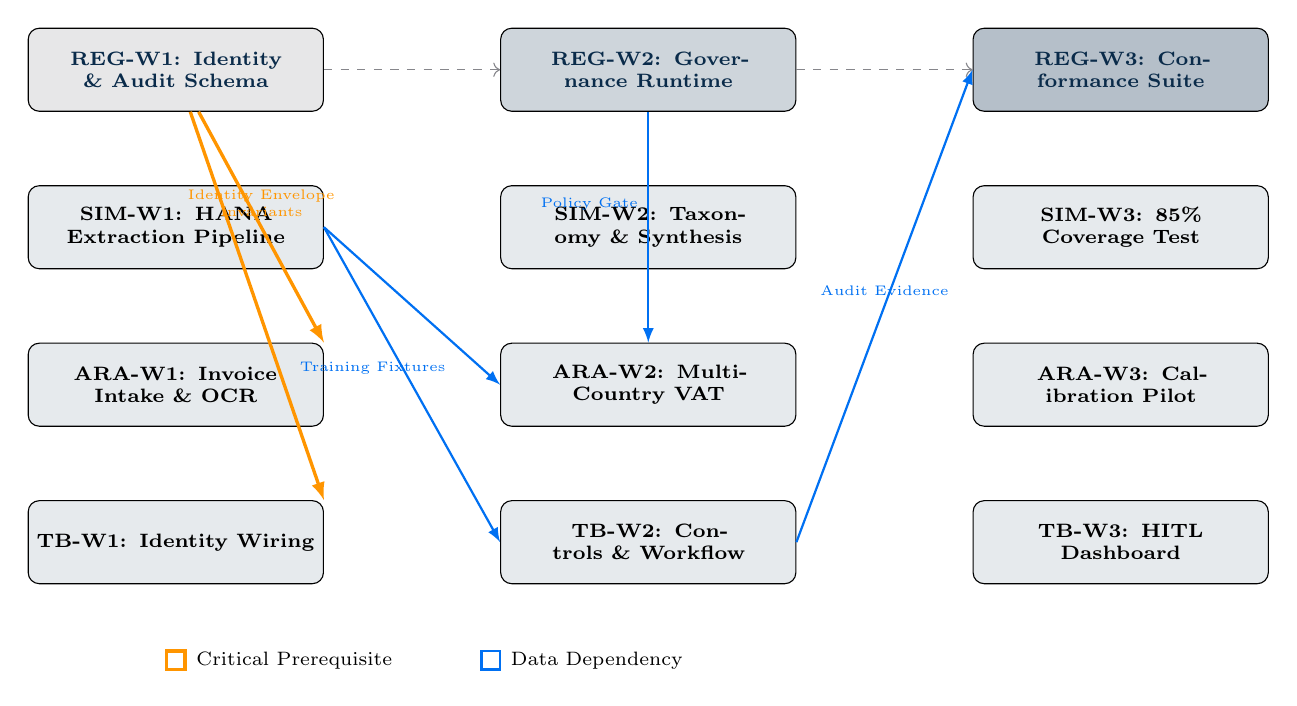
\begin{tikzpicture}[
node distance=1.5cm,
auto,
wavebox/.style={rectangle, draw, rounded corners, fill=sapmidnight!10, text width=10em, text centered, minimum height=3em, font=\scriptsize\bfseries},
dep/.style={->, >=latex, thick, sapblue},
critical/.style={->, >=latex, very thick, sapamber}
]
% --- Wave 1: Foundations ---
\node (r1) [wavebox, fill=sapgrey!20] {\textcolor{sapmidnight}{REG-W1: Identity \& Audit Schema}};
\node (s1) [wavebox, below of=r1, yshift=-0.5cm] {SIM-W1: HANA Extraction Pipeline};
\node (a1) [wavebox, below of=s1, yshift=-0.5cm] {ARA-W1: Invoice Intake \& OCR};
\node (t1) [wavebox, below of=a1, yshift=-0.5cm] {TB-W1: Identity Wiring};

% --- Wave 2: Core Build-out ---
\node (r2) [wavebox, right of=r1, xshift=4.5cm, fill=sapmidnight!20] {\textcolor{sapmidnight}{REG-W2: Governance Runtime}};
\node (s2) [wavebox, right of=s1, xshift=4.5cm] {SIM-W2: Taxonomy \& Synthesis};
\node (a2) [wavebox, right of=a1, xshift=4.5cm] {ARA-W2: Multi-Country VAT};
\node (t2) [wavebox, right of=t1, xshift=4.5cm] {TB-W2: Controls \& Workflow};

% --- Wave 3: Hardening ---
\node (r3) [wavebox, right of=r2, xshift=4.5cm, fill=sapmidnight!30] {\textcolor{sapmidnight}{REG-W3: Conformance Suite}};
\node (s3) [wavebox, right of=s2, xshift=4.5cm] {SIM-W3: 85\% Coverage Test};
\node (a3) [wavebox, right of=a2, xshift=4.5cm] {ARA-W3: Calibration Pilot};
\node (t3) [wavebox, right of=t2, xshift=4.5cm] {TB-W3: HITL Dashboard};

% --- Cross-Domain Dependencies (The Critical Path) ---
\draw [critical] (r1) -- node [above, font=\tiny, align=center] {Identity Envelope\\Invariants} (a1.north east);
\draw [critical] (r1) -- (t1.north east);
\draw [dep] (s1.east) -- node [above, font=\tiny, xshift=-0.5cm] {Training Fixtures} (t2.west);
\draw [dep] (s1.east) -- (a2.west);
\draw [dep] (r2.south) -- node [left, font=\tiny, yshift=0.3cm] {Policy Gate} (a2.north);
\draw [dep] (t2.east) -- node [above, font=\tiny] {Audit Evidence} (r3.west);

% --- Wave Transitions ---
\draw [->, dashed, sapgrey] (r1.east) -- (r2.west);
\draw [->, dashed, sapgrey] (r2.east) -- (r3.west);

% --- Legend ---
\node[draw, sapamber, very thick, label=right:\scriptsize Critical Prerequisite] at (0,-7.5) {};
\node[draw, sapblue, thick, label=right:\scriptsize Data Dependency, xshift=4cm] at (0,-7.5) {};

\end{tikzpicture}
\caption{Cross-specification dependency graph: The blueprint for platform rollout.}
\end{figure}

\section{Inter-Domain Prerequisite Matrix}

\begin{table}[htbp]
\centering
\footnotesize
\caption{Normative Cross-Domain Prerequisites.}
\label{tab:prerequisites}
\begin{tabularx}{\textwidth}{@{}l l l X@{}}
\toprule
\textbf{Target Task} & \textbf{Prerequisite} & \textbf{Ref ID} & \textbf{Rationale} \\
\midrule
\rowcolor{sapmidnight!5}
\textbf{ARA-W1} & REG-W1 (Identity) & \texttt{REG-IDENTITY-01} & Invoice intake must be audit-traced from Day 1. \\
\textbf{TB-W2}  & SIM-W1 (Extraction) & \texttt{SIM-EXTRACT-01} & Anomaly detection requires HANA schema metadata. \\
\rowcolor{sapmidnight!5}
\textbf{REG-W2} & SIM-W1 (Registry) & \texttt{SIM-REGISTRY-01} & Governance monitoring relies on the schema registry. \\
\textbf{ARA-W2} & REG-W2 (Pillar 1) & \texttt{REG-MGF-P1} & VAT release is an HITL gate governed by MAS Pillar 1. \\
\rowcolor{sapmidnight!5}
\textbf{TB-W3}  & ARA-W2 (Posted Invoices) & \texttt{ARA-AP-POST} & Review dashboard depends on posted AP data from Arabic domain. \\
\bottomrule
\end{tabularx}
\end{table}

\begin{adrbox}{Dependency Enforcement}
Implementation agents are strictly forbidden from "Fast-Forwarding" into Wave 2 if Wave 1 critical prerequisites (marked in \textcolor{sapamber}{\textbf{Gold}}) are in a \textsc{gap} or \textsc{partial} state.
\end{adrbox}



\end{document}
